\documentclass[male,czech,api_bc]{kitheses}
\usepackage{ifthen}

\usepackage{amsmath,amssymb}
\usepackage{graphics}
\usepackage{color}
\usepackage{array}
\usepackage{longtable}
\usepackage{afterpage}
\usepackage{microtype}  

\usepackage{graphicx}
\usepackage{float}

\iftutex
\else
\usepackage{etoolbox}
\makeatletter
\newcommand\my@hsyphen{-}
\newcommand\my@apostroph{'}
\patchcmd\select@language{-}{\my@hyphen }{}{}
\patchcmd\select@language{'}{\my@apostroph }{}{}
\makeatother
\fi

\iftutex
	\usepackage{fontspec}  
	\setmainfont{Libertinus Serif}
	\setsansfont{Libertinus Sans}
	\setmonofont[Scale=MatchLowercase]{Source Code Pro}
	\usepackage{unicode-math}
	\setmathfont{Libertinus Math}
\else
	\usepackage[utf8]{inputenc} 
	\usepackage[T1]{fontenc}
	\usepackage{libertinus}
	\renewcommand{\ttdefault}{pxtt}
\fi

\usepackage{csquotes} 
\usepackage[style=iso-numeric,shortnumeration=true]{biblatex}
\addbibresource{references.bib}


\usepackage{listings}
\usepackage{xcolor}
\lstset{ %
  language=Python,              
  basicstyle=\small\ttfamily,    
  backgroundcolor=\color{white},
  showspaces=false,             
  showstringspaces=false,       
  showtabs=false, 
  frame=single,   
  tabsize=3,                    
  breaklines=true,              
  breakatwhitespace=false, 
  keywordstyle=\bfseries\color{blue},       
  commentstyle=\rmfamily\color{gray},       
  stringstyle=\itshape\color{teal},   
}
\usepackage[printonlyused]{acronym}

\newcommand{\nazevcz}{Systém pro monitorování a analýzu dopravy pomocí počítačového vidění}   
\newcommand{\nazeven}{System for Traffic Monitoring and Analysis using Computer Vision}     
\newcommand{\autor}{Patrik Poklop}           
\newcommand{\rok}{\the\year}                
\newcommand{\vedouci}{Ing. Roman Vaibar Ph.D., MBA}         
\newcommand{\vedouciDAT}{Ing. Romanu Vaibarovi, Ph.D., MBA}
% zvětšuje o 23% vertikální okraje v tabulkách
\renewcommand{\arraystretch}{1.23}
% nastavení pro záhlaví (co nelze udělat v cls souboru)
\renewcommand{\chaptermark}[1]{\markboth{\arabic{chapter}. #1}{}}
\pagestyle{fancy}
% nastavení odkazů
\usepackage{url} % formátování URL, příkaz \url
%\usepackage{varioref} % lepší interní odkazy na obrázky, apod. příkaz \vref
%\usepackage{cleveref}
\usepackage[unicode=true,pdfusetitle,
 bookmarks=true,
 breaklinks=false,pdfborder={0 0 1},backref=false,colorlinks=false]{hyperref} % hypertextové odkazy v PDF
\newcommand{\UV}[1]{\quotedblbase#1\textquotedblleft}
% odstraňte pokud vám vadí absence zarovnání dole 
\raggedbottom

\begin{document}

\thispagestyle{empty}
\begin{center}
{
\LARGE
\univerzita\\[16pt]
\fakulta
}

\vspace{2cm}
\resizebox{8.42cm}{!}{%
\ifthenelse{\boolean{czech}}
{
\includegraphics{LOGO_PRF_CZ_RGB_standard.jpg}}
{
\includegraphics{LOGO_PRF_EN_RGB_standard.jpg}}}

\vspace{2cm}
{
\Huge\sffamily
\nazevcz\par
\vspace{0.6cm}
\Large\scshape \ifthenelse{\boolean{bc}}{bakalářská}{diplomová} práce
}
\end{center} 
 
\vfill
{
\large
\begin{tabular}{>{\bfseries}rl}
    Vypracoval: 	& \autor\\
    Vedoucí práce: 	& \vedouci\\
&\\
Studijní program:       & \program\\
\ifthenelse{\boolean{api}}{Studijní obor:          & Api\\}{}
\end{tabular} 
}
\vspace{1.5cm}
\begin{center}
  \Large\scshape   Ústí nad Labem \rok
\end{center}

\cleardoublepage
\thispagestyle{empty}
\pagecolor{yellow}
{\Large Namísto žlutých stránek vložte digitálně podepsané zadání kvalifikační práce poskytnuté vedoucím katedry.\\\
Zadání musí zaujímat právě dvě strany.
}

Zadání je nutno vložit jako PDF pomocí některého nástroje, který umožňuje editaci dokumentů (se zachováním
elektronického podpisu).

V Linuxe lze například použít příkaz \texttt{pdftk}.

\clearpage
\thispagestyle{empty}
\afterpage{\nopagecolor}
~
\clearpage

\thispagestyle{empty} 
{\bfseries Prohlášení}

\vspace{0.5cm}
Prohlašuji, že jsem tuto \ifthenelse{\boolean{bc}}{bakalářskou}{diplomovou} práci vypracoval\ifthenelse{\boolean{feminum}}{a}{}
samostatně a použil\ifthenelse{\boolean{feminum}}{a}{}
jen pramenů, které cituji a uvádím v přiloženém seznamu literatury.

\vspace{0.5em}

Byl\ifthenelse{\boolean{feminum}}{a}{} jsem seznámen\ifthenelse{\boolean{feminum}}{a}{} 
s tím, že se na moji práci vztahují práva a povinnosti vyplývající ze
zákona č. 121/2000 Sb., ve znění zákona č. 81/2005 Sb., autorský zákon, zejména se
skutečností, že Univerzita Jana Evangelisty Purkyně v Ústí nad Labem má právo na uzavření
licenční smlouvy o užití této práce jako školního díla podle § 60 odst. 1 autorského zákona, a
s tím, že pokud dojde k užití této práce mnou nebo bude poskytnuta licence o užití jinému
subjektu, je Univerzita Jana Evangelisty Purkyně v Ústí nad Labem oprávněna ode mne
požadovat přiměřený příspěvek na úhradu nákladu, které na vytvoření díla vynaložila, a to
podle okolností až do jejich skutečné výše.

\vspace{2em}

V Ústí nad Labem dne \today   \hfill Podpis: \makebox[4cm][s]{\dotfill}

\cleardoublepage
\thispagestyle{empty}
~
\vfill

\begin{flushright}
    Děkuji vedoucímu práce {\vedouciDAT}\\ 
    za neocenitelné rady a pomoc při tvorbě bakalářské práce.
\end{flushright}

\cleardoublepage

\textsc{\nazevcz}

\textbf{Abstrakt:}

Tato bakalářská práce se zabývá návrhem, implementací a vyhodnocením systému pro monitorování a analýzu dopravy pomocí metod počítačového vidění. Cílem práce je vytvořit funkční prototyp zařízení schopného v reálném čase analyzovat videozáznam z dopravní lokality, detekovat a klasifikovat účastníky provozu, jako jsou vozidla, chodci a cyklisté, a zaznamenávat jejich průjezdy a průchody definovanou oblastí. Navržený systém je realizován na platformě Raspberry Pi s využitím AI akcelerátoru a moderních detekčních modelů. Součástí práce je také softwarová aplikace pro ukládání a vizualizaci získaných dat. Funkčnost a přesnost systému jsou ověřeny pomocí experimentů v reálném prostředí a porovnáním s manuálním pozorováním.

\textbf{Klíčová slova:} počítačové vidění, monitorování dopravy, detekce objektů, Edge AI, Raspberry Pi

\bigskip

\textsc{\nazeven}

\textbf{Abstract:}

This bachelor’s thesis focuses on the design, implementation, and evaluation of a system for traffic monitoring and analysis using computer vision methods. The aim of the thesis is to develop a functional prototype capable of real-time video analysis of a traffic scene, including detection and classification of traffic participants such as vehicles, pedestrians, and cyclists, and counting their movements across a defined area. The proposed system is implemented on the Raspberry Pi platform using an AI accelerator and modern object detection models. The thesis also includes the development of a software application for data storage and visualization. The functionality and accuracy of the system are verified through experiments conducted in real-world conditions and by comparison with manual observations.

\textbf{Keywords:} computer vision, traffic monitoring, object detection, Edge AI, Raspberry Pi

\tableofcontents

\clearpage

\addcontentsline{toc}{chapter}{Seznam zkratek} %
\chapter*{Seznam zkratek} 
\begin{acronym}[PCIe] 
    \acro{AI}{Artificial Intelligence (Umělá inteligence)}
    \acro{ALPR}{Automatic License Plate Recognition (Automatické rozpoznávání registračních značek)}
    \acro{ARM}{Advanced RISC Machine (Architektura energeticky úsporných procesorů)}
    \acro{CPU}{Central Processing Unit (Centrální procesorová jednotka)}
    \acro{DeepSORT}{Deep Simple Online and Realtime Tracking (Rozšíření algoritmu SORT o hluboké učení)}
    \acro{Edge AI}{Edge Artificial Intelligence (Umělá inteligence na okraji sítě / lokální zpracování modelů na koncových zařízeních)}
    \acro{FPS}{Frames Per Second (Počet zpracovaných snímků za sekundu)}
    \acro{GDPR}{General Data Protection Regulation (Obecné nařízení o ochraně osobních údajů)}
    \acro{GPU}{Graphics Processing Unit (grafický procesor)}
    \acro{HTTP}{Hypertext Transfer Protocol (Hypertextový přenosový protokol)}
    \acro{ID}{Identifier (Identifikátor / Unikátní označení objektu)}
    \acro{IoU}{Intersection over Union (Metrika prostorového překryvu detekcí)}
    \acro{IP}{Internet Protocol (Internetový protokol pro přenos dat po síti)}
    \acro{MOT}{Multiple Object Tracking (Víceobjektové sledování)}
    \acro{NPU}{Neural Processing Unit (Neuronový procesor pro akceleraci umělé inteligence)}
    \acro{ONVIF}{Open Network Video Interface Forum (Globální standard pro komunikaci IP kamer)}
    \acro{PCIe}{Peripheral Component Interconnect Express (Vysokorychlostní počítačová sběrnice)}
    \acro{PoE}{Power over Ethernet (Technologie pro napájení zařízení po datovém kabelu)}
    \acro{R-CNN}{Region-based Convolutional Neural Network (Architektura dvoufázové detekce objektů)}
    \acro{RAM}{Random Access Memory (operační paměť s přímým přístupem)}
    \acro{ROI}{Region of Interest (Oblast zájmu / sledovaný výřez v obraze)}
    \acro{RTSP}{Real-Time Streaming Protocol (Síťový protokol pro přenos streamovaného videa)}
    \acro{SORT}{Simple Online and Realtime Tracking (Algoritmus pro online sledování v reálném čase)}
    \acro{SSD}{Single Shot MultiBox Detector (Architektura jednofázové detekce objektů)}
    \acro{YOLO}{You Only Look Once (Architektura jednofázové detekce objektů)}
\end{acronym}

\addchap{Úvod}
Rostoucí intenzita dopravy představuje jednu z hlavních výzev současných měst a aglomerací. Zvyšující se počet vozidel klade vysoké nároky nejen na propustnost samotné dopravní infrastruktury, ale také na bezpečnost silničního provozu a celkovou kvalitu života obyvatel. Efektivní řízení a plánování dopravy proto vyžaduje přesná, kontinuálně sbíraná a aktuální data. Tradiční metody získávání těchto dat, jako je například manuální sčítání dopravy, jsou však časově i personálně náročné a náchylné k chybám. Vzniká tak silná potřeba automatizace celého procesu.

V reakci na tyto potřeby a v rámci širšího rozvoje konceptu chytrých měst (z angl. \textit{Smart Cities}) se jako vysoce efektivní řešení ukazuje využití moderních technologií. Klíčovým nástrojem se v tomto kontextu stává počítačové vidění v kombinaci s umělou inteligencí. Kamerové systémy doplněné o algoritmy strojového učení poskytují flexibilní a škálovatelné řešení pro automatizované sledování, vyhodnocování a predikci dopravních jevů. Jejich hlavní výhodou je možnost nasazení v reálném prostředí stávajících komunikací bez nutnosti rozsáhlých a nákladných stavebních zásahů do infrastruktury.

S překotným rozvojem výpočetních technologií a hardwarové miniaturizace se v této oblasti navíc stále více prosazuje přístup tzv. \ac{Edge AI} (umělá inteligence na okraji sítě). Zpracování rozsáhlých obrazových dat díky tomu již nemusí probíhat ve vzdálených datacentrech, ale je realizováno přímo na okrajových zařízeních v místě sběru dat. Využití kompaktních jednodeskových počítačů doplněných o specializované hardwarové AI akcelerátory umožňuje dramatické snížení latence, zvýšení ochrany citlivých osobních údajů a minimalizaci závislosti na stabilním internetovém připojení či cloudových službách. V dopravních aplikacích, kde je vyžadováno spolehlivé zpracování v reálném čase, je tento přístup zásadní.

Cílem této bakalářské práce je navrhnout, implementovat a otestovat plně funkční systém pro automatické sčítání a analýzu dopravního provozu, postavený na principech \ac{Edge AI}. Práce se zaměřuje na detekci, sledování a klasifikaci různých účastníků provozu – primárně vozidel, chodců a cyklistů – v definované lokalitě s využitím moderních detekčních modelů pro víceobjektové sledování. Důraz je kladen na praktickou realizaci celého řešení na dostupném okrajovém zařízení a na následné vyhodnocení přesnosti detekce i sčítání z reálných videozáznamů dopravy.

Text práce je strukturován do šesti hlavních kapitol. První, část teoretická poskytuje ucelený přehled v oblastech počítačového vidění, metod detekce a sledování objektů a existujících systémů pro monitorování dopravy. Následně se věnuje specifikům \ac{Edge AI} a etickým aspektům sběru dat. Druhá kapitola přibližuje celkový návrh architektury systému, včetně zdůvodnění výběru hardwarových komponent. Třetí kapitola detailně popisuje samotnou implementaci řešení od přípravy vývojového prostředí až po ukládání a vizualizaci nasbíraných dat. Čtvrtá a pátá kapitola jsou dedikovány testování systému v reálných scénářích, vyhodnocení přesnosti modelu a diskuzi nad dosaženými výsledky. Závěrečná kapitola pak shrnuje zjištěné poznatky a nastiňuje možnosti budoucího rozvoje vytvořené aplikace.

\chapter{Teoretická část}

\section{Sledování a počítání objektů}
Sledování objektů v obrazových sekvencích a videu představuje klíčovou nadstavbu nad samotnou detekcí objektů. Zatímco detekce umožňuje lokalizovat a klasifikovat objekty v jednotlivých izolovaných snímcích, sledování zajišťuje jejich konzistentní identifikaci napříč časem. Tato vlastnost je vysoce heterogenní a zásadní zejména v dopravních aplikacích, kde je pro komplexní analýzu nutné sledovat plynulý pohyb vozidel, určovat jejich trajektorie, rychlost nebo měřit přesný počet průjezdů daným úsekem komunikace~\cite{szeliski_computer_vision, zhou_traffic_survey_2024}.

\subsection{Víceobjektové sledování (MOT)}
Víceobjektové sledování (\acs{MOT}, z angl. \textit{\acl{MOT}})\acused{MOT} se zabývá současným sledováním většího počtu dynamických objektů ve scéně. Hlavním cílem je přiřazení unikátních a časově konzistentních identifikátorů (Unique \ac{ID}) každému objektu při jeho prvním výskytu ve scéně. Tento identifikátor je následně udržován po celou dobu výskytu entity ve sledované sekvenci, což umožňuje spojování detekcí mezi jednotlivými snímky a rekonstrukci trajektorie objektu v čase. V dopravních monitorovacích systémech nachází \acs{MOT} uplatnění zejména při analýze dopravních toků, odhadu hustoty provozu, detekci anomálií nebo sledování pohybu vozidel a chodců na komplexních křižovatkách~\cite{zhou_traffic_survey_2024}.

Tento proces je ve většině moderních architektur realizován pomocí přístupu „detekce před sledováním“ (z angl. \textit{Tracking-by-Detection}). Systém nejprve v každém snímku identifikuje objekty pomocí detekčního konvolučního modelu a následně provádí asociaci těchto detekcí mezi po sobě jdoucími snímky na základě kombinace prostorových, časových a vzhledových charakteristik. Správná správa těchto identifikátorů je kritická pro následné navazující úlohy, jako je statistické počítání objektů nebo pokročilá analýza jejich chování~\cite{szeliski_computer_vision}.

\begin{figure}[H]
    \centering
    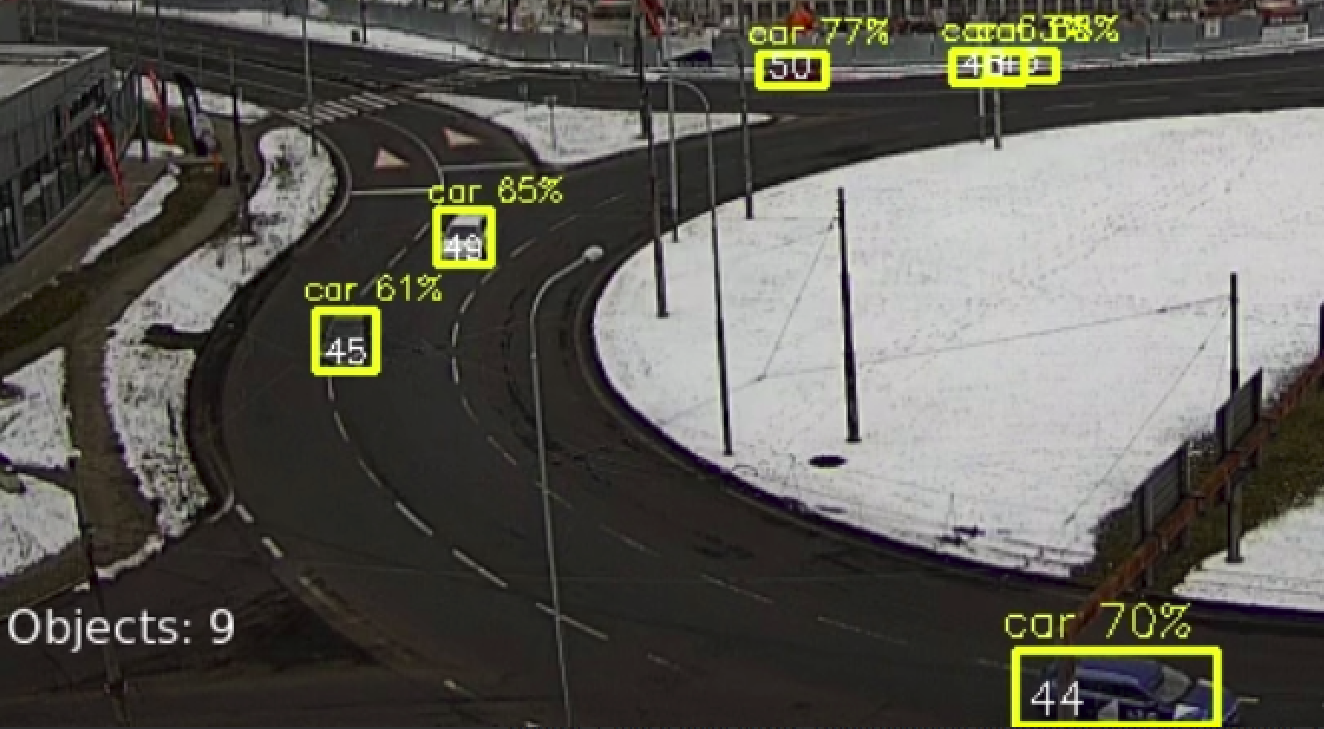
\includegraphics[width=0.9\textwidth]{images/own_tracking.png}
    \caption{Ukázka víceobjektového sledování vozidel s přiřazenými časově konzistentními identifikátory (vlastní zpracování, akcelerátor Hailo-8)}
    \label{fig:own_tracking}
\end{figure}

Jak je znázorněno na obrázku~\ref{fig:own_tracking}, implementovaný systém umožňuje stabilní sledování většího množství objektů v reálném čase, přičemž každému vozidlu zůstává zachováno jeho unikátní číslo i při pohybu napříč snímanou scénou.

\subsection{Algoritmy pro sledování objektů}
Mezi nejpoužívanější a nejefektivnější přístupy pro sledování objektů v reálném čase patří algoritmy SORT a DeepSORT. Tyto metody jsou oblíbené zejména pro svou nízkou výpočetní náročnost, vysokou propustnost a snadnou integraci s moderními detekčními modely, jako je rodina modelů \acs{YOLO} (z angl. \textit{\acl{YOLO}})\acused{YOLO}~\cite{redmon_yolo_2016}.


\subsubsection{SORT}
Algoritmus \acs{SORT} (z angl. \textit{\acl{SORT}})\acused{SORT} je postaven na kombinaci dvou klíčových komponent: Kalmanova filtru\footnote{Kalmanův filtr je rekurzivní matematický algoritmus, který ze série nepřesných a zašuměných měření (v tomto případě historických detekcí z kamery) odhaduje aktuální a predikuje budoucí stav dynamického systému (například polohu, směr a rychlost jedoucího vozidla).} a Maďarského algoritmu pro datovou asociaci. Kalmanův filtr slouží k predikci budoucí polohy objektu v následujícím snímku na základě lineárního pohybového modelu. Stav každého sledovaného objektu je definován vektorově pomocí souřadnic středu ohraničujícího obdélníku, jeho plochy (měřítka), poměru stran a jejich příslušných rychlostí změn v čase.

Jakmile jsou v novém snímku získány čerstvé detekce, nastupuje Maďarský algoritmus, který řeší optimalizační úlohu přiřazení predikovaných poloh k reálným novým detekcím. Jako nákladová funkce (metrika vzdálenosti) se zde využívá překryv ohraničujících obdélníků vyjádřený pomocí metriky (\acs{IoU}, z angl. \textit{\acl{IoU}})\acused{IoU}. Díky této matematické přímočarosti dosahuje SORT extrémní rychlosti zpracování, avšak jeho zásadní nevýhodou je nestabilita při dlouhodobějších překryvech (okluzích) objektů, kdy absence vizuální informace často vede ke ztrátě stopy a fatálnímu selhání přiřazení \ac{ID}.~\cite{SORT_original_2016}.

\begin{figure}[H]
    \centering
    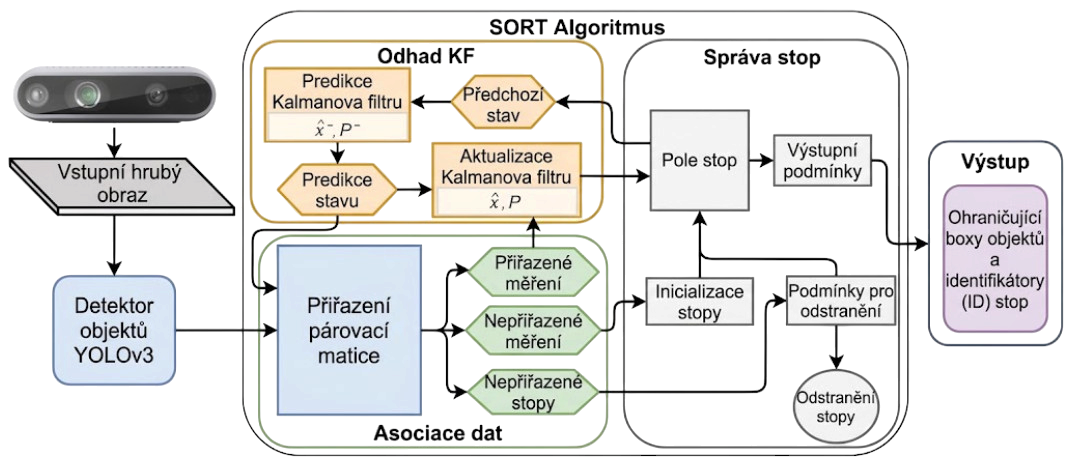
\includegraphics[width=1\textwidth]{images/sort_algorithm_principe_CZ.png}
    \caption{Celkový přehled a princip fungování sledovacího algoritmu SORT (vlastní překlad, adaptováno z~\cite[s.~5]{pereira2022sort}).}
    \label{fig:sort_overview}
\end{figure}

%Na obrázku~\ref{fig:sort_overview} je detailně znázorněna celá pracovní smyčka (z angl. \textit{pipeline}) algoritmu SORT~\cite{SORT_original_2016}, která se nezávisle opakuje s každým novým obrazovým snímkem. Podle blokového schématu lze celý proces logicky rozdělit do tří na sebe navazujících fází:

%\begin{enumerate}
%    \item \textbf{Odhad Kalmanovým filtrem (z angl. \textit{KF Estimation}):} Tato část schématu představuje paměť systému. Na základě předchozího stavu (\textit{Previous State}) algoritmus provede matematickou predikci (\textit{Kalman Filter Prediction}), čímž získá odhadovanou polohu sledovaných objektů v aktuálním čase (\textit{State Prediction}).
%    \item \textbf{Asociace dat (z angl. \textit{Data Association}):} Do tohoto bloku vstupují jak odhadnuté polohy z Kalmanova filtru, tak zcela nové detekce z modelu YOLO. Úkolem párovací matice (\textit{Cost Matrix Matching}) je optimálně spojit tyto dva vstupy pomocí metriky \acs{IoU}. Výstupem jsou tři možné stavy: úspěšně spárovaná měření (\textit{Matched Measurement}), nové detekce bez historie (\textit{Unmatched Measurement}) a existující stopy, ke kterým se nenašla nová detekce (\textit{Unmatched Tracks}).
%    \item \textbf{Správa stop (z angl. \textit{Track Management}):} V závěrečné fázi systém reaguje na výsledky předchozí asociace. Spárovaná měření aktualizují Kalmanův filtr a udržují se v poli aktivních stop (\textit{Array of Tracks}). Z nespárovaných měření, což typicky představuje nově příchozí vozidla, se inicializují stopy nové (\textit{Track Initialization}). Nespárované stopy, tedy vozidla, která pravděpodobně opustila scénu, jsou po splnění stanovených podmínek ze systému odstraněny (\textit{Track Delete}). Validní stopy jsou následně propuštěny na finální výstup (\textit{Output}).
%\end{enumerate}

Na obrázku~\ref{fig:sort_overview} je detailně znázorněna celá pracovní smyčka (z angl. \textit{pipeline}) algoritmu SORT~\cite{SORT_original_2016}, která se nezávisle opakuje s každým novým obrazovým snímkem. Podle blokového schématu lze celý proces logicky rozdělit do tří na sebe navazujících fází:

\begin{enumerate}
    \item \textbf{Odhad KF:} Tato část schématu představuje paměť systému. Na základě předchozího stavu (\textit{Předchozí stav}) algoritmus provede matematickou predikci (\textit{Predikce Kalmanova filtru}), čímž získá odhadovanou polohu sledovaných objektů v aktuálním čase (\textit{Predikce stavu}).
    
    \item \textbf{Asociace dat:} Do tohoto bloku vstupují jak odhadnuté polohy z Kalmanova filtru, tak zcela nové detekce z modelu YOLO. Úkolem párovací matice (\textit{Přiřazení párovací matice}) je optimálně spojit tyto dva vstupy pomocí metriky \acs{IoU}. Výstupem jsou tři možné stavy: úspěšně spárovaná měření (\textit{Přiřazené měření}), nové detekce bez historie (\textit{Nepřiřazené měření}) a existující stopy, ke kterým se nenašla nová detekce (\textit{Nepřiřazené stopy}).
    
    \item \textbf{Správa stop:} V závěrečné fázi systém reaguje na výsledky předchozí asociace. Spárovaná měření aktualizují Kalmanův filtr a udržují se v poli aktivních stop (\textit{Pole stop}). Z nespárovaných měření, což typicky představuje nově příchozí vozidla, se inicializují stopy nové (\textit{Inicializace stopy}). Nespárované stopy, tedy vozidla, která pravděpodobně opustila scénu, jsou po splnění stanovených podmínek ze systému odstraněny (\textit{Odstranění stopy}). Validní stopy jsou následně propuštěny na finální výstup (\textit{Výstup}).
\end{enumerate}

\subsubsection{DeepSORT}
Algoritmus DeepSORT (z angl. \textit{\acl{DeepSORT}})\acused{DeeSORT} vznikl jako přímá reakce na slabá místa původního algoritmu SORT v komplexních a hustých scénách. Rozšiřuje čistě geometrické a prostorové přiřazování o integraci hlubokých konvolučních neuronových sítí, které jsou vytrénovány pro extrakci vizuálních vzhledových příznaků (z angl. \textit{deep appearance descriptors}). Pro každý detekovaný objekt je vygenerován charakteristický vektor (embedding), který reprezentuje jeho vizuální identitu.

Při samotné asociaci dat pak DeepSORT kombinuje dvě metriky: Mahalanobisovu vzdálenost, která reflektuje pohybovou konzistenci na základě Kalmanova filtru, a kosinovou vzdálenost, jež vyhodnocuje shodu vizuálních příznaků s historií daného objektu. Propojení těchto informací probíhá pomocí kaskádového párování (\textit{matching cascade}). Tento kombinovaný přístup dramaticky zvyšuje robustnost sledování v hustém dopravním provozu, kde dochází k častému vzájemnému zakrývání vozidel, a prokazatelně minimalizuje množství chyb typu záměny identity (\textit{\ac{ID} switches})~\cite{wojke_deepsort_2017}.

\begin{figure}[H]
    \centering
    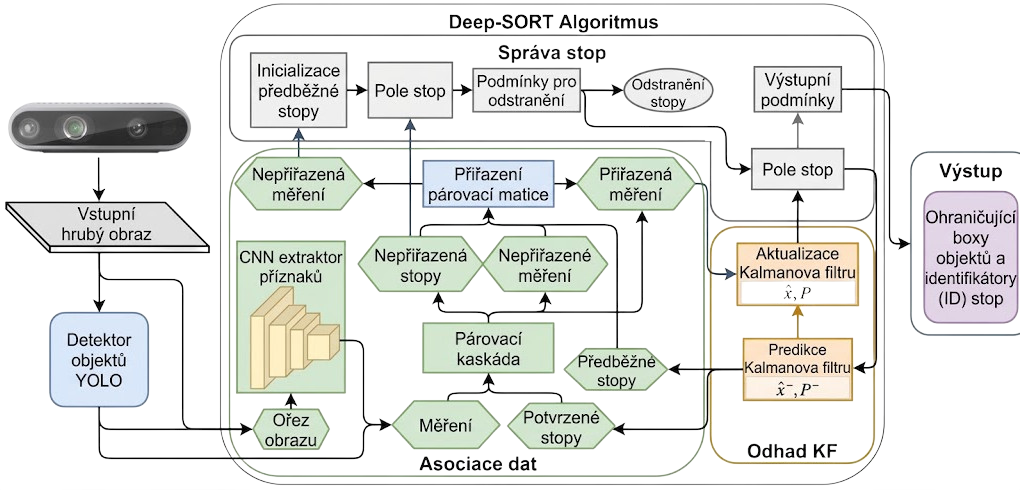
\includegraphics[width=1\textwidth]{images/deepsort_algorithm_principe_CZ.png}
    \caption{Blokové schéma architektury sledovacího algoritmu DeepSORT a jeho rozhodovacích kroků (vlastní překlad, adaptováno z ~\cite[s.~7]{pereira2022sort})}
    \label{fig:deepsort_overview}
\end{figure}

Na obrázku~\ref{fig:deepsort_overview} je detailně znázorněna architektura a datový tok algoritmu Deep-SORT. Podle blokového schématu lze celý proces rozdělit do následujících klíčových fází, které se vykonávají s každým novým snímkem:

\begin{enumerate}
    \item \textbf{Extrakce příznaků a predikce polohy:} Vstupní obraz (\textit{Vstupní hrubý obraz}) je nejprve zpracován detektorem objektů, ze kterého jsou získány obrazové výřezy jednotlivých vozidel (\textit{Ořez obrazu}). Tyto výřezy následně zpracovává konvoluční neuronová síť (\textit{CNN extraktor příznaků}), jež extrahuje unikátní vizuální příznaky. Souběžně s tím modul odhadu (\textit{Odhad KF}) provádí matematickou predikci budoucí polohy pomocí Kalmanova filtru (\textit{Predikce Kalmanova filtru}).
    
    \item \textbf{Asociace dat:} Tento centrální modul kombinuje nová měření obohacená o vizuální příznaky (\textit{Měření}) a potvrzené stopy z minulosti (\textit{Potvrzené stopy}). Klíčovým inovačním prvkem oproti původnímu algoritmu SORT je kaskádové párování (\textit{Párovací kaskáda}), které prioritně využívá právě vizuální podobnost. Objekty a měření, které kaskáda nedokáže spojit (\textit{Nepřiřazené stopy} a \textit{Nepřiřazená měření}), jsou zachyceny a předány do klasické párovací matice (\textit{Přiřazení párovací matice}), jež funguje jako záloha využívající standardní prostorový překryv.
    
    \item \textbf{Správa stop a aktualizace:} Výstupy z asociace dat se dělí do tří směrů. Úspěšně spárovaná měření (\textit{Přiřazená měření}) jsou využita k okamžité aktualizaci Kalmanova filtru (\textit{Aktualizace Kalmanova filtru}). Zcela nová detekovaná vozidla, která nemají historii (\textit{Nepřiřazená měření}), zakládají v systému nové, zatím nepotvrzené stopy (\textit{Inicializace předběžné stopy}). Správa stop následně kontroluje celé pole aktivních záznamů (\textit{Pole stop}). Vozidla, jež dlouhodobě chybí a splní podmínky pro smazání (\textit{Podmínky pro odstranění}), jsou ze systému odstraněna (\textit{Odstranění stopy}). Stopy splňující výstupní kritéria (\textit{Výstupní podmínky}) jsou předány na finální výstup v podobě souřadnic a unikátních identifikátorů (\textit{Výstup}).
\end{enumerate}

\subsection{Metody sčítání objektů}
Samotné automatické sčítání objektů v dopravním proudu bezprostředně navazuje na výsledky získané z MOT. Namísto prosté kumulace detekcí v jednotlivých samostatných snímcích, která by vedla k masivnímu nadhodnocení výsledků (například z důvodu vícenásobného započítání téhož stojícího či pomalu jedoucího vozidla), se využívá analýzy časoprostorových trajektorií jednoznačně identifikovaných objektů~\cite{zhou_traffic_survey_2024}.

V praxi se pro automatizované sčítání a kategorizaci využívají dva primární koncepční přístupy:
\begin{itemize}
    \item \textbf{Virtuální čára (z angl. \textit{Virtual Line}):} Jedná se o nejrozšířenější a výpočetně nejméně náročnou metodu pro sčítání vozidel v konkrétních jízdních pruzích či směrech. V obrazovém prostoru je definována úsečka fungující jako detekční brána. Systém v každém kroku kontroluje, zda vektor trajektorie konkrétního objektu (typickky reprezentovaný středovým nebo spodním bodem jeho ohraničujícího obdélníku) protnul tuto linii. V okamžiku detekce průsečíku je inkrementováno počítadlo pro daný směr jízdy. Tento přístup je vysoce efektivní pro stanovení okamžité intenzity dopravy na liniových úsecích komunikací~\cite{zhou_traffic_survey_2024}.
    \item \textbf{Oblast zájmu (z angl. \ac{ROI}):} Alternativní přístup spočívá ve vymezení uzavřené polygonální nebo obdélníkové zóny přímo v digitálním obraze. Sledovaný objekt je zaregistrován a statisticky započítán buď v momentě vstupu do této definované oblasti, nebo při jejím opuštění. Tento princip se využívá především v situacích, kde je nutné sledovat celkovou obsazenost určitého vyhrazeného prostoru (např. plochy křižovatek, odbočovací pruhy nebo parkoviště) či analyzovat průměrnou dobu zdržení vozidel v daném segmentu~\cite{szeliski_computer_vision, zhou_traffic_survey_2024}.
\end{itemize}

\begin{figure}[H]
    \centering
    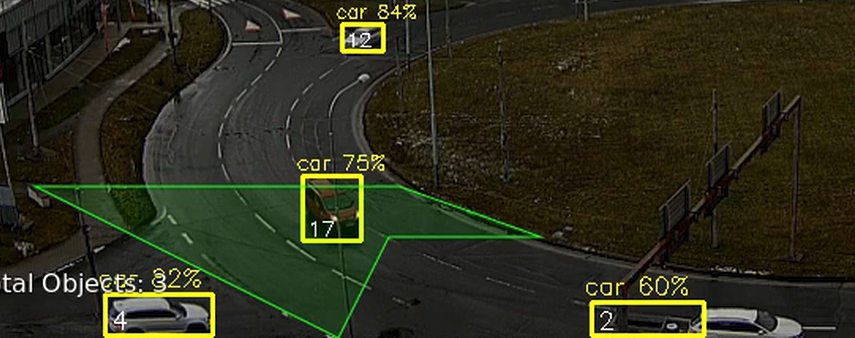
\includegraphics[width=1\textwidth]{images/own_objects_tracking.png}
    \caption{Definice analytické oblasti zájmu (\acs{ROI}) pomocí polygonu v praktické implementaci sledovacího systému (vlastní zpracování, akcelerátor Hailo-8).}
    \label{fig:own_roi_polygon}
\end{figure}

Jak ukazuje obrázek~\ref{fig:own_roi_polygon}, zatímco na rovných úsecích komunikací často postačuje k detekci průjezdu jednoduchá virtuální čára, složitější dopravní uzly, jakými jsou kruhové objezdy, vyžadují robustnější přístup. V rámci předložené implementace je proto oblast zájmu (\acs{ROI}) definována jako nepravidelný n-úhelník (polygon). Tento geometrický útvar je v systému konstruován pomocí přesné sady 2D souřadnic (vrcholů) definovaných v obrazovém prostoru předzpracovaného snímku.

Proces samotného sčítání a vyhodnocování trajektorií je následně založen na průběžném výpočtu prostorového průniku (z angl. \textit{spatial intersection}). Systém v každém snímku kontinuálně extrahuje polohu sledovaných objektů, jež jsou typicky reprezentovány středovým bodem (centroidem) jejich ohraničujícího obdélníku. Jakmile vyhodnocovací algoritmus detekuje, že se tento referenční bod vozidla nachází přímo uvnitř definované polygonové zóny (což matematicky odpovídá úloze bodu v polygonu, tzv. \textit{Point-in-Polygon}), je vozidlo okamžitě započítáno do celkové statistiky dopravy. Tento moment je na obrázku názorně zachycen u objektu s identifikátorem 17. Tento plošný přístup výrazně eliminuje chyby spojené s nepřesnostmi detekce na hranách a umožňuje spolehlivé sčítání i při zakřivených a překrývajících se trajektoriích.


\section{Počítačové vidění pro analýzu dopravy}
Počítačové vidění (z angl. \textit{Computer Vision}) představuje interdisciplinární oblast informatiky, která se zabývá automatickou analýzou statických snímků a videozáznamů. Jeho hlavním cílem je extrakce relevantních a sémantických informací z vizuálních vstupů. V oblasti moderních dopravních systémů je počítačové vidění využíváno zejména v aplikacích dopravního dohledu, proaktivního řízení provozu a při automatické analýze dopravní propustnosti. Kamerové systémy umožňují kontinuální sledování dopravních toků, detekci anomálních situací nebo identifikaci konkrétních vozidel a jejich registračních značek~\cite{szeliski_computer_vision, zhou_traffic_survey_2024}.

\subsection{Předzpracování obrazu}
Předzpracování obrazu představuje nezbytný přípravný krok před samotnou aplikací detekčních modelů. Cílem je zlepšení kvality vstupních dat, potlačení digitálního šumu a optimalizace celkové výpočetní zátěže. 

V dopravních aplikacích je surový videozáznam z kamery často výpočetně příliš objemný a obsahuje velké množství irelevantních informací (např. oblohu, okolní budovy, chodníky). Prvním logickým krokem je proto definice oblasti zájmu (\acs{ROI}, z angl. \textit{\acl{ROI}})\acused{ROI}. Softwarové oříznutí nebo zavedení masky zaručí, že systém analyzuje pouze samotnou vozovku. To nejen radikálně snižuje objem zpracovávaných dat, ale také eliminuje falešné detekce, jako jsou například zaparkovaná vozidla mimo zorné pole křižovatky.

Následně musí být upravený obraz transformován do formátu, který striktně vyžaduje architektura neuronové sítě. Jedná se primárně o \textbf{škálování (z angl. \textit{resizing})} na fixní rozlišení (typicky $640 \times 640$). Aby při změně velikosti nedošlo k deformaci poměru stran, což by zhoršilo schopnost sítě rozeznat tvar a proporce vozidla, využívá se běžně technika zvaná \textit{letterboxing}. Ta zmenší obraz proporcionálně a chybějící prostor (okraje) doplní neutrální barvou. 

Poslední rutinní fází je \textbf{normalizace barev}. Hodnoty jednotlivých pixelů, které standardně nabývají celočíselných hodnot 0 až 255, jsou převedeny na desetinná čísla v intervalu 0,0 až 1,0. Tento krok stabilizuje a výrazně urychluje matematické výpočty (násobení matic) uvnitř umělé neuronové sítě~\cite{szeliski_computer_vision}. I přes tuto důkladnou datovou optimalizaci však analýza obrazu zůstává nesmírně výpočetně náročná, což představuje hlavní výzvu při nasazení na okrajových zařízeních.

\begin{figure}[H]
    \centering
    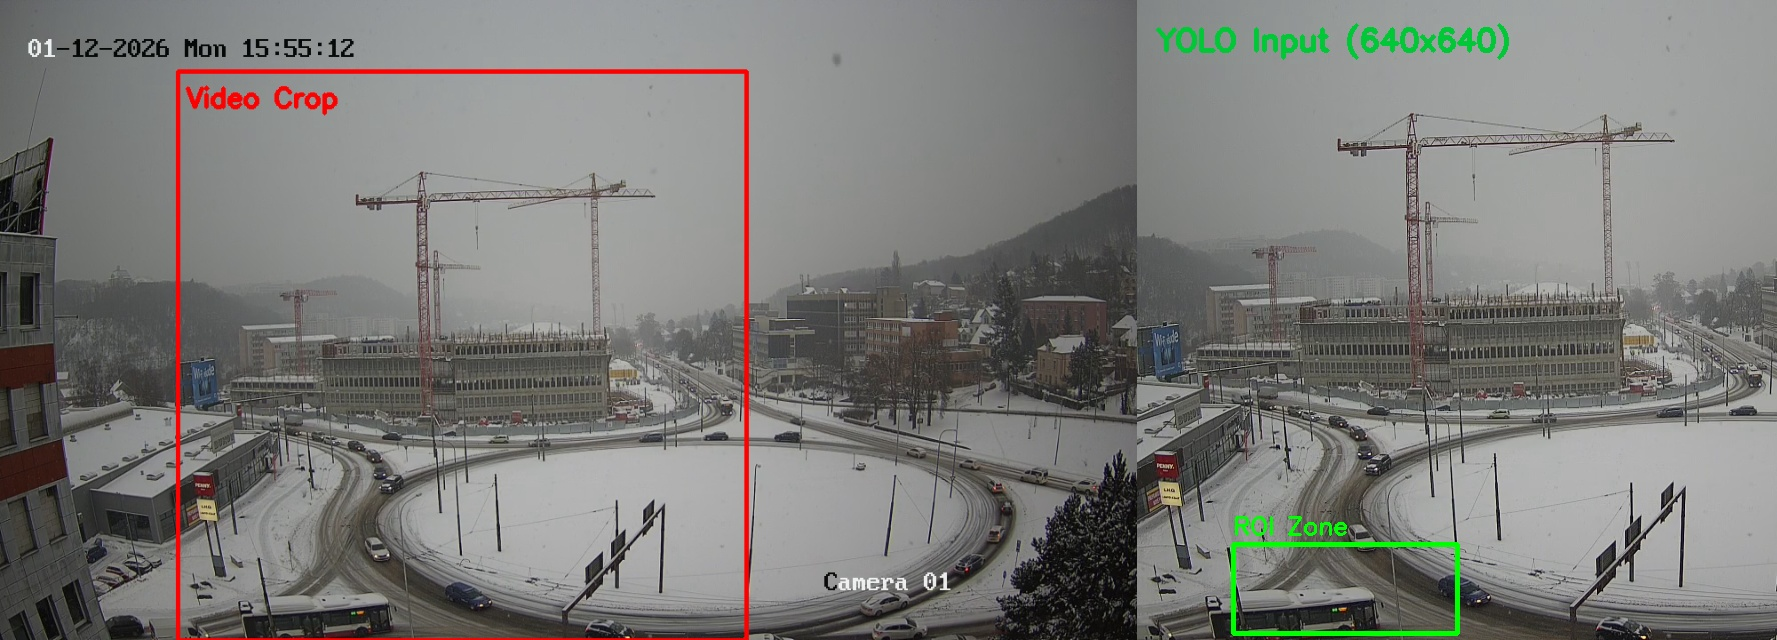
\includegraphics[width=\textwidth]{images/preprocessing_gstreamer.jpg}
    \caption{Příklad dvoufázového vymezení oblasti zájmu, hardwarový ořez vlevo a softwarová analytická zóna vpravo (vlastní zpracování).}
    \label{fig:image_preprocessing}
\end{figure}

Jak ukazuje obrázek~\ref{fig:image_preprocessing}, předzpracování obrazového toku hraje klíčovou roli v optimalizaci celého systému. Namísto výpočetně náročnějších metod (jako je doplňování černých pruhů u \textit{letterboxingu}) je v navrženém systému využit přímý prostorový ořez obrazu (z angl. \textit{crop}). Levá část obrázku znázorňuje zdrojový snímek, který byl v rámci datovodu nejprve naškálován na rozlišení $1280\times720$ pixelů. Červený obdélník v něm přesně vymezuje hranice hardwarového ořezu ten je definován počátečními souřadnicemi $x=200, y=80$ s pevnou šířkou a výškou $640$ pixelů. 

Pravá část následně představuje fyzicky vyříznutý čtverec, jenž svými rozměry ($640\times640$) nativně odpovídá požadavkům vstupní vrstvy modelu YOLO. Je nutné zdůraznit, že tento hardwarový ořez slouží výhradně k obrazové přípravě dat před vstupem do modelu. Samotná analytická oblast zájmu (\acs{ROI}), která určuje, kde reálně dochází k detekci a sčítání vozidel, je v systému definována až následně. Na pravé části obrázku je tato aplikační logika vizualizována zeleným obdélníkem. Jeho poloha je v aplikačním kódu dynamicky vypočítávána pomocí relativních souřadnic vůči velikosti předzpracovaného výstupu (v tomto konkrétním případě $x=96, y=544, w=224, h=90$). Oddělením těchto dvou fází je do neuronové sítě propuštěn čistší datový tok, přičemž analytika si zachovává plnou flexibilitu.


%\subsection{Zpracování obrazu s nízkou latencí}
%Při nasazení v reálné dopravní infrastruktuře je kladen extrémní důraz na rychlost vyhodnocování a efektivní využití dostupných hardwarových prostředků. Namísto obecného a často zavádějícího pojmu „reálný čas“ je v kontextu této práce definován přísný časový požadavek – navržený algoritmus musí dokázat kompletně zpracovat jeden snímek v čase kratším než 1/20 sekundy (což odpovídá zpracování do 50~ms, potažmo propustnosti 20 snímků za sekundu).

%Tyto časové limity jsou kritické zejména u vestavěných systémů a okrajových zařízení (z angl. \textit{edge devices}), která nedisponují výpočetní silou velkých datacenter. Splnění těchto limitů zaručuje, že nedojde ke ztrátě informací o rychle jedoucích vozidlech ani k nežádoucímu hromadění zpožděných dat ve vyrovnávacích pamětech~\cite{hailo_alpr_2024}. Dosažení těchto nekompromisních časových milníků je tak přímo podmíněno výběrem extrémně rychlé a optimalizované architektury detekční sítě.

\subsection{Základní úlohy počítačového vidění}
V rámci analýzy dopravy a návrhu inteligentní dopravní infrastruktury se počítačové vidění opírá o tři základní, na sebe úzce navazující úlohy:

\begin{itemize}
    \item \textbf{Detekce objektů:} Zaměřuje se na samotnou lokalizaci objektů v obraze. Výstupem této úlohy jsou obvykle ohraničující obdélníky (z angl. \textit{bounding boxes}), které vymezují prostorovou polohu nalezených entit. V dopravních aplikacích se jedná především o detekci vozidel, chodců nebo cyklistů.
    \item \textbf{Klasifikace objektů:} Představuje úlohu, při které je již detekovanému objektu přiřazena předem definovaná třída na základě jeho vizuálních charakteristik. V praxi se využívá například pro rozlišení, zda je detekované vozidlo osobní automobil, nákladní vůz nebo autobus~\cite{szeliski_computer_vision}.
    \item \textbf{Sledování objektů:} Umožňuje analyzovat pohyb detekovaných a klasifikovaných objektů napříč po sobě jdoucími snímky video sekvence. Slouží k odhadu trajektorií, predikci směru a výpočtu rychlosti pohybu~\cite{zhou_traffic_survey_2024}.
\end{itemize}

\begin{figure}[H]
    \centering
    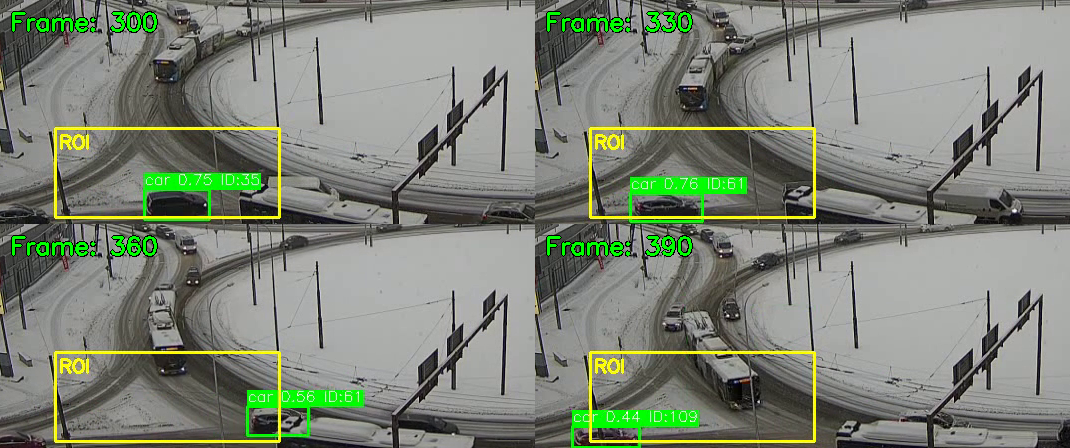
\includegraphics[width=1\textwidth]{images/tracking_grid_final.png}
    \caption{Časová sekvence čtyř snímků demonstrující kontinuální sledování objektů a vyhodnocování jejich polohy vůči definované zóně (ROI). Systém úspěšně udržuje \ac{ID} u projíždějícího automobilu a dynamicky registruje nová vozidla (vlastní zpracování, inference na GPU).}
    \label{fig:object_tracking_example}
\end{figure}

Jak je názorně ukázáno na obrázku~\ref{fig:object_tracking_example}, propojení úlohy detekce a sledování umožňuje systému přidělit jednotlivým vozidlům unikátní identifikátory (\ac{ID}) a kontinuálně je sledovat v čase. Obrázek zachycuje sekvenci čtyř po sobě jdoucích snímků s pevným rozestupem 30 rámečků (snímky 300, 330, 360 a 390). Vzhledem k tomu, že zdrojové video je zpracováváno frekvencí 15 snímků za sekundu (FPS), představuje časový krok mezi každým zobrazeným dílčím obrázkem přesně 2 sekundy reálného času (celá mřížka tak mapuje celkem 6 sekund dopravního provozu). Pro každé detekované vozidlo systém neustále vypočítává středový bod (centroid) jeho ohraničujícího obdélníku. Zásadní analytickou podmínkou je, že vozidlo je do statistik průjezdů aktivně zahrnuto pouze tehdy, nachází-li se tento vypočítaný střed fyzicky uvnitř definované oblasti zájmu (žlutý obdélník \acs{ROI}).

Plynulý průjezd a spolehlivost sledování jsou prokazatelně demonstrovány na osobním automobilu (označeném jako \textit{car ID:61}). Toto vozidlo je zachyceno ve sledované zóně \acs{ROI} ve snímku 330, přičemž o dvě sekundy později (snímek 360) si systém navzdory jeho pohybu napříč křižovatkou úspěšně udržuje jeho původní \ac{ID}. Z mřížky je rovněž jasně patrné, jak algoritmus dynamicky reaguje na celkovou obměnu vozidel ve scéně. Zatímco na prvním snímku (300) zónou projíždí předchozí vozidlo s \ac{ID} 35, na posledním snímku (390) do \acs{ROI} zleva vstupuje další automobil, kterému systém okamžitě a správně přiděluje nové, dosud nepoužité \ac{ID} (109). Tento holistický přístup, kombinující striktní prostorové omezení analytickou zónou a konzistentní sledování identity napříč snímky, je v dopravních aplikacích naprosto klíčový pro zabránění falešnému vícenásobnému započítání téhož objektu.

\section{Přehled detekčních modelů}
V posledních letech dominují oblasti detekce objektů architektury hlubokých konvolučních neuronových sítí (CNN). Pro nasazení na výpočetně omezených okrajových zařízeních se historicky osvědčily zejména modely z rodiny SSD a YOLO, které patří do kategorie tzv. jednofázových detektorů (z angl. \textit{one-stage detectors}). Tyto modely dokáží obraz zpracovat během jediného průchodu sítí, čímž splňují výše zmíněné požadavky na nízkou latenci.

Architektura \acs{SSD} (z angl. \textit{\acl{SSD}})\acused{SSD} detekuje objekty tak, že využívá hustou sadu předem definovaných kotevních obdélníků (z angl. \textit{anchor boxes}) o různých poměrech stran a velikostech. Predikce probíhá na několika mapách příznaků s různým rozlišením současně, což modelu teoreticky umožňuje lépe zachytit objekty nejrůznějších velikostí~\cite{szeliski_computer_vision}.

%Ačkoliv \ac{SSD} dosahuje stabilní přesnosti, v kontextu nasazení na vysoce omezeném hardwaru nedosahuje takové efektivity jako inovativnější přístupy. Z tohoto důvodu byl pro praktickou implementaci v této bakalářské práci zvolen model z rodiny YOLO. Tento model nabízí bezkonkurenční poměr mezi přesností detekce a propustností snímků a disponuje vynikající softwarovou podporou pro následnou kompilaci a optimalizaci na dedikovaných AI akcelerátorech.

\subsection{Model YOLO}
Ačkoliv SSD dosahuje stabilní přesnosti, naprostou revoluci v efektivitě přinesla architektura \acs{YOLO} (z angl. \textit{\acl{YOLO}})\acused{YOLO}, která od základů transformovala přístup k počítačovému vidění. Namísto dvoufázového generování návrhů oblastí (jako u starších sítí \acs{R-CNN} (z angl. \textit{\acl{R-CNN}})\acused{R-CNN}) formuluje detekci jako jedinou, \textit{end-to-end} regresní úlohu~\cite{redmon_yolo_2016}.

\begin{figure}[H]
    \centering    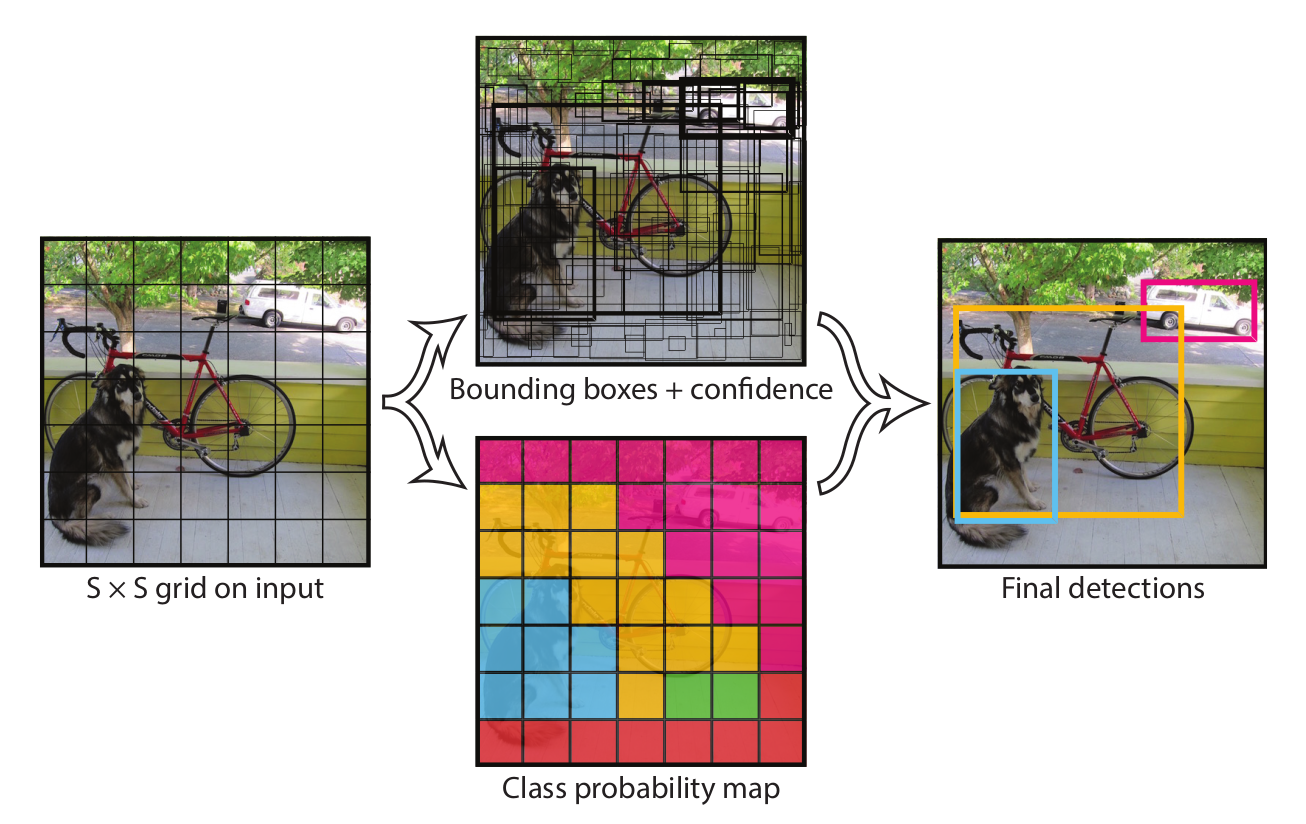
\includegraphics[width=1\textwidth]{images/yolo_v1_diagram.png}
    \caption{Základní princip detekce modelu YOLO využívající rozdělení obrazu do mřížky (převzato z~\cite[s.~2]{redmon_yolo_2016})}
    \label{fig:detection_principe}
\end{figure}

Jak ukazuje obrázek~\ref{fig:detection_principe}, vstupní obraz je nejprve virtuálně rozdělen do mřížky $S \times S$. Pokud střed hledaného objektu spadne geometricky do konkrétní buňky této mřížky, stává se tato konkrétní buňka plně zodpovědnou za jeho detekci. Každá buňka následně predikuje fixní počet $B$ ohraničujících obdélníků, míru spolehlivosti (z angl. \textit{confidence score}) pro tyto obdélníky a pravděpodobnosti zařazení do $C$ různých tříd. Celkový výstup sítě je tak elegantně zakódován do jediného tenzoru o rozměrech $S \times S \times (B \cdot 5 + C)$.

\begin{figure}[H]
    \centering
    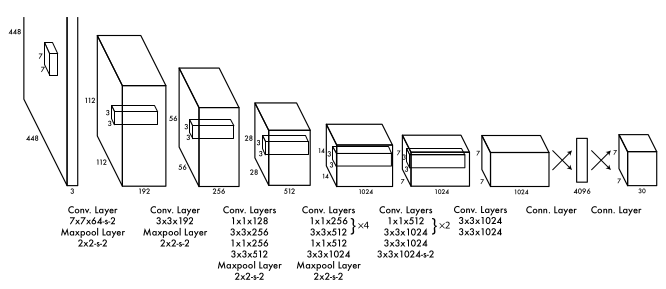
\includegraphics[width=1\textwidth]{images/yolo_model_conv.png}
    \caption{Vnitřní architektura modelu YOLO znázorňující sekvenci konvolučních a plně propojených vrstev (převzato z~\cite[s.~3]{redmon_yolo_2016})}
    \label{fig:yolo_arch}
\end{figure}
Na obrázku~\ref{fig:yolo_arch} je detailně znázorněna topologie vrstev původního modelu YOLO, jejíž architektura byla přímo inspirována modelem GoogLeNet\footnote{GoogLeNet (známý také pod označením Inception v1) je průlomová architektura hluboké konvoluční neuronové sítě od společnosti Google, která v roce 2014 zvítězila v prestižní soutěži počítačového vidění ImageNet (ILSVRC). Vyznačuje se velmi vysokou výpočetní efektivitou.}. Systém na svém vstupu přijímá obraz o přesném rozlišení $448 \times 448$ pixelů. Samotná síť se skládá z 24 konvolučních vrstev, které slouží k postupné a hluboké extrakci vizuálních příznaků z obrazu (od jednoduchých hran až po komplexní tvary vozidel). Za nimi následují 2 plně propojené vrstvy (z angl. \textit{fully connected layers}), jež získané příznaky agregují a generují finální predikční tenzor o rozměrech $7 \times 7 \times 30$.

Klíčovým inovačním prvkem této architektury je zařazení střídavých redukčních konvolučních vrstev s filtrem $1 \times 1$. Tyto vrstvy fungují jako informační úzká hrdla (z angl. \textit{bottlenecks}) – efektivně zmenšují prostor příznaků z předchozích vrstev, čímž drasticky redukují množství potřebných matematických operací bez zásadní ztráty kontextu. Moderní varianty modelů z rodiny YOLO jsou pro účely přesné objektové detekce standardně trénovány a vyhodnocovány na rozsáhlém datasetu COCO\footnote{\href{https://www.kaggle.com/datasets/erennik/coconames}{COCO dataset}} (z angl. \textit{Common Objects in Context})~\cite{lin_coco_2014}. Tento dataset obsahuje stovky tisíc detailně anotovaných snímků reálných scén a plně definuje 80 základních tříd objektů, což detekčnímu modelu poskytuje vysoce robustní výchozí základ pro spolehlivé rozpoznávání různorodých účastníků dopravního provozu (osobní automobily, autobusy, nákladní vozy či chodce).

\section{Systémy pro monitorování dopravy}
Monitorování dopravy představuje klíčovou součást moderních inteligentních dopravních systémů. Jeho primárním cílem je kontinuální získávání informací o dopravním provozu, jako je intenzita dopravy, průměrná rychlost vozidel, detekce kongescí nebo výskyt nestandardních dopravních událostí. Tyto agregované informace jsou následně využívány pro aktivní řízení dopravy, strategické plánování městské infrastruktury a zvyšování celkové bezpečnosti silničního provozu~\cite{zhou_traffic_survey_2024}.

\subsection{Tradiční metody dopravního monitoringu}
Tradiční metody monitorování dopravy jsou historicky založeny převážně na fyzických kontaktních senzorech nebo manuálním sběru dat. Mezi jejich hlavní výhody patří relativně přímočará implementace a dlouhodobé ověření v praxi, zásadní nevýhodou je však jejich omezená flexibilita, neschopnost poskytovat hlubší kontext a vysoké náklady na instalaci i následnou údržbu.

Jednou z nejstarších metod je manuální sčítání dopravy, při kterém jsou dopravní prostředky zaznamenávány lidským pozorovatelem. Tento přístup je extrémně časově i personálně náročný, náchylný k lidským chybám způsobeným únavou a je naprosto nevhodný pro kontinuální dlouhodobý monitoring dopravního provozu~\cite{zhou_traffic_survey_2024}.

Další široce rozšířenou technologií jsou indukční smyčky zabudované přímo do povrchu vozovky, které detekují přítomnost kovového podvozku vozidla na základě změny elektromagnetického pole. Ačkoliv poskytují relativně spolehlivá data o prostých průjezdech vozidel, jejich instalace vyžaduje destruktivní zásah do vozovky, což omezuje dopravu, a podléhají rychlému opotřebení vlivem zátěže a povětrnostních podmínek~\cite{zhou_traffic_survey_2024}.

Pro monitorování rychlosti a vzdálenosti jsou rovněž hojně využívány radarové a lidarové senzory. Tyto technologie dosahují vysoké přesnosti i za zhoršené viditelnosti, avšak jejich nevýhodou jsou vysoké pořizovací náklady a omezené možnosti vizuální klasifikace jednotlivých typů objektů (např. obtížné rozlišení mezi malým motocyklem a chodcem)~\cite{zhou_traffic_survey_2024}.

% pridat obrazek tuzka papir, mobil s kategoriema
\subsection{Moderní kamerové systémy}
S raketovým rozvojem počítačového vidění a dostupnosti vysokého výpočetního výkonu se v dopravní infrastruktuře stále častěji prosazují kamerové systémy založené na analýze obrazových dat. Na rozdíl od jednorozměrných dat z indukčních smyček umožňují kamerové systémy získávat z jednoho zařízení bohaté, vícerozměrné informace o celé dopravní scéně, včetně přesného typu vozidel, jejich trajektorií nebo anomálního chování účastníků provozu~\cite{szeliski_computer_vision}.

Mezi hlavní výhody těchto systémů patří vysoká flexibilita (změna sledované oblasti často vyžaduje pouze softwarovou úpravu virtuálních čar, nikoliv překopání vozovky) a možnost využití jedné kamery pro paralelní běh více analytických úloh. Nevýhodou kamerových systémů jsou naopak jejich limity spojené s kvalitou vstupních obrazových dat. Výkon detekčních a sledovacích algoritmů může být negativně ovlivněn prudkými změnami světelných podmínek, nepříznivým počasím (mlha, hustý déšť) nebo vzájemným vizuálním překrýváním objektů ve scéně. Tyto faktory představují výzvu zejména v hustém městském provozu~\cite{zhou_traffic_survey_2024}.

\subsubsection{Vstupní zařízení kamerových systémů}

\begin{figure}[H]
    \centering
    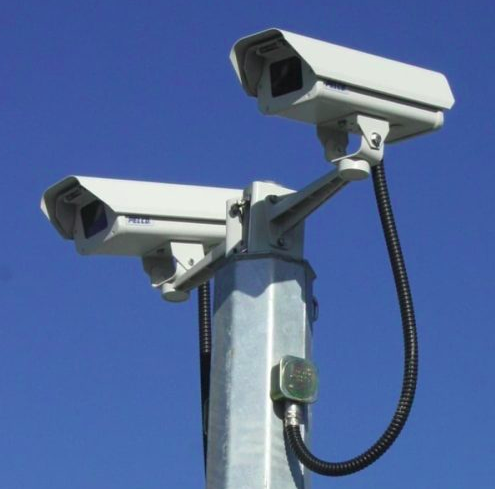
\includegraphics[width=0.5\textwidth]{images/traffic_camera.jpg}
    \caption{Typické umístění dohledových \ac{IP} kamer na sloupu infrastruktury. Toto neinvazivní řešení poskytuje stabilní obrazový tok pro následnou detekci a inferenci na okrajových zařízeních (převzato z~\cite{zdroj_kamera}).}
    \label{fig:traffic_camera}
\end{figure}

Pro zajištění kvalitního obrazového vstupu, který je pro algoritmy počítačového vidění kritický, se v moderních \ac{Edge AI} systémech využívají primárně dva typy snímacích zařízení, jež přímo reflektují potřeby vývoje i reálného nasazení v dopravní infrastruktuře:

\begin{itemize}
    \item \textbf{\ac{IP} kamery:} Představují současný standard v budování chytrých měst. Tato zařízení nejenže snímají obraz, ale rovnou ho digitálně kódují a odesílají prostřednictvím počítačové sítě (nejčastěji pomocí protokolů \ac{RTSP} nebo \ac{ONVIF}). Jejich obrovskou výhodou je snadná integrace do existující síťové infrastruktury a možnost napájení přes jeden datový kabel (technologie \ac{PoE}). Pro účely detekce na okrajových zařízeních poskytují \ac{IP} kamery ideální a stabilní zdroj datového toku, ze kterého systém v reálném čase extrahuje jednotlivé snímky pro inferenci.
    
    \item \textbf{Kamerové moduly s přímým rozhraním (např. senzory Sony IMX):} Jedná se o kompaktní kamerové moduly navržené pro přímé hardwarové připojení k jednodeskovým počítačům (jako je platforma Raspberry Pi) pomocí vysokorychlostní sběrnice MIPI CSI. Zásadní výhodou tohoto řešení je minimální latence, jelikož surová obrazová data putují ze snímače rovnou do operační paměti výpočetního zařízení bez nutnosti jakéhokoliv síťového kódování a dekódování. Tyto senzory představují vysoce efektivní nástroj pro prototypování a autonomní nasazení analytických uzlů bez nutnosti budování složité lokální sítě.
\end{itemize}

% obrazky kamer pridat
\subsection{Existující řešení a projekty}
% popsat pouze cloud reseni a edge reseni
V současnosti existuje na trhu řada komerčních i výzkumných řešení zaměřených na monitorování dopravy. Většinu těchto systémů lze z architektonického hlediska rozdělit na dvě hlavní větve: centralizovaná cloudová řešení a distribuovaná řešení na okrajích sítě (Edge AI).

Komerční platformy často spoléhají na to, že kamerové systémy na křižovatkách slouží pouze jako pasivní snímače, které odesílají nepřetržitý videostream do vzdálených cloudových datových center. Zde se za pomoci masivního výpočetního výkonu provádí přesná analytika a trasování. Ačkoliv je tento přístup vysoce přesný, naráží na limity v podobě vysokých nároků na propustnost síťového připojení, latenci a v neposlední řadě představuje bezpečnostní riziko z hlediska ochrany osobních údajů (GDPR), jelikož citlivé videozáznamy plynule opouštějí lokální infrastrukturu.

Moderním a stále preferovanějším trendem jsou proto systémy implementované přímo na okrajových zařízeních (z angl. \textit{edge devices}). Zde je kladen důraz na efektivní využití úsporných výpočetních prostředků a AI akcelerátorů přímo v místě sběru dat~\cite{li_edge_ai_2020}.

%\textbf{Srovnání s navrhovaným řešením:} 
%Navrhované řešení zpracovávané v rámci této bakalářské práce plně reflektuje trend Edge AI. Od mohutných komerčních systémů se odlišuje svým důrazem na modularitu, využitím otevřených softwarových technologií (open-source) a lokálním zpracováním. Systém je navržen tak, aby se dokázal připojit ke standardnímu síťovému toku z běžně dostupné IP kamery a pomocí dedikovaného hardwarového akcelerátoru prováděl analýzu v reálném čase lokálně. Díky tomu nedochází k odesílání obrazových dat mimo zabezpečenou síť, ukládají se výhradně anonymizovaná textová a statistická data (počty průjezdů, časy, směry), což razantně snižuje síťovou zátěž a přirozeně řeší problematiku GDPR.

\section{Edge AI a vestavěné systémy}
Koncept tzv. Edge AI označuje moderní architektonický přístup, při kterém jsou výpočetně náročné úlohy umělé inteligence realizovány přímo na okrajových zařízeních v těsné blízkosti zdroje dat, nikoliv v centrálním cloudovém prostředí. Tento přesun logiky umožňuje dramatické snížení latence, omezení objemu přenášených dat a mnohem efektivnější využití dostupných síťových zdrojů~\cite{li_edge_ai_2020}.

\subsection{Požadavky na zpracování s nízkou latencí}
Při nasazení v reálné dopravní infrastruktuře je kladen extrémní důraz na rychlost vyhodnocování a efektivní využití dostupných hardwarových prostředků. Namísto obecného a často zavádějícího pojmu „reálný čas“ je v kontextu této práce definován přísný časový požadavek – navržený algoritmus musí dokázat kompletně zpracovat jeden snímek v čase kratším než 1/20 sekundy (což odpovídá zpracování do 50~ms, potažmo propustnosti 20 snímků za sekundu).

Tyto časové limity jsou kritické zejména u vestavěných systémů a okrajových zařízení (z angl. \textit{edge devices}), která nedisponují masivní výpočetní silou velkých datacenter. Splnění těchto limitů zaručuje, že nedojde ke ztrátě informací o rychle jedoucích vozidlech ani k nežádoucímu hromadění zpožděných dat ve vyrovnávacích pamětech~\cite{hailo_alpr_2024}.

\subsection{Zpracování obrazu na okraji sítě}
Zpracování obrazu na okraji sítě (z angl. \textit{Edge Computing}) představuje přímou alternativu ke klasickému centralizovanému zpracování. V případě tradičního cloudového řešení musí být surová obrazová data (často tvořící masivní datový tok) neustále odesílána do vzdáleného datového centra. Naproti tomu edge přístup analyzuje video přímo na zařízení, ke kterému je kamera připojena.

Hlavním rozdílem a zároveň největším benefitem je eliminace zpoždění sítě (latence). Lokální inference hlubokých neuronových sítí přímo na okrajovém zařízení nejenže zajišťuje okamžitou odezvu, ale zároveň razantně zvyšuje celkovou robustnost systému. V případě dočasného výpadku internetového připojení může systém nadále plnohodnotně fungovat, lokálně ukládat agregovaná textová data o dopravě a odeslat je až po obnovení spojení~\cite{li_edge_ai_2020}.

\begin{figure}[H]
    \centering
    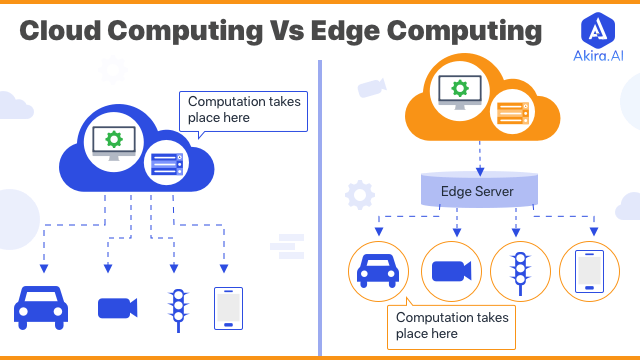
\includegraphics[width=0.9\textwidth]{images/akira-ai-cloud-computing-vs-edge-computing.png}
    \caption{Porovnání architektury a datových toků u edge a cloudového zpracování (převzato z~\cite{akira_edge_cloud})}
    \label{fig:edge_vs_cloud}
\end{figure}

Na obrázku~\ref{fig:edge_vs_cloud} je schematicky znázorněn rozdíl mezi oběma přístupy. Cloud computing se spoléhá na centrální servery, což vytváří úzké hrdlo na síťové vrstvě. Edge computing naopak přesouvá výpočetní logiku (inferenci) až na samotný okraj sítě k senzorům, což garantuje vysokou propustnost a okamžité vyhodnocování.

\subsection{Hardwarové AI akcelerátory}
AI akcelerátory, často označované jako \acs{NPU} (z angl. \textit{\acl{NPU}})\acused{NPU}, jsou specializované integrované obvody navržené primárně pro efektivní provádění tenzorových výpočtů. Na rozdíl od univerzálních centrálních procesorů (\acs{CPU}) jsou tyto čipy na hardwarové úrovni optimalizovány pro masivní paralelní zpracování maticových operací, jež tvoří matematický základ hlubokých konvolučních sítí.

V kontextu Edge AI jsou tyto akcelerátory naprosto nezbytné, protože překonávají tzv. von Neumannovo úzké hrdlo. Běžné procesory ztrácejí obrovské množství času a energie neustálým přesouváním mezivýsledků mezi výpočetními jednotkami a hlavní pamětí. Akcelerátory tento problém eliminují tím, že udržují data co nejblíže samotným výpočetním jádrům. Umožňují tak nasazení složitých detekčních a sledovacích modelů na energeticky úsporných a prostorově omezených vestavěných zařízeních, a to při zachování propustnosti nutné pro plynulou analýzu dopravy bez závislosti na výkonných serverových farmách~\cite{hailo_alpr_2024, hailo_architecture_2026}.

\subsection{Platforma Raspberry Pi a akcelerace pomocí Hailo-8}
Platforma Raspberry Pi \footnote{\href{https://rpishop.cz}{Rpishop}} představuje rodinu kompaktních jednodeskových počítačů (z angl. \textit{Single-Board Computers}), které se staly standardem pro prototypování a vývoj vestavěných systémů. Její hlavní vlastností a výhodou je nízká pořizovací cena, obrovská komunitní podpora, stabilní operační systém (založený na linuxovém jádře) a především široká škála hardwarových rozhraní pro připojení periferních senzorů a modulů~\cite{raspberrypi_docs_2024}.

Zásadním omezením samotné architektury Raspberry Pi je však její hrubý výpočetní výkon. Integrovaný procesor postavený na architektuře \acs{ARM} není schopen v reálném čase zpracovávat náročné úlohy počítačového vidění, a už vůbec ne zajišťovat běh hlubokých neuronových sítí. Z tohoto důvodu je pro nasazení v systémech monitorování dopravy nezbytné doplnit základní desku o externí výpočetní modul~\cite{raspberrypi_ai_kit}.

\begin{figure}[H]
    \centering
    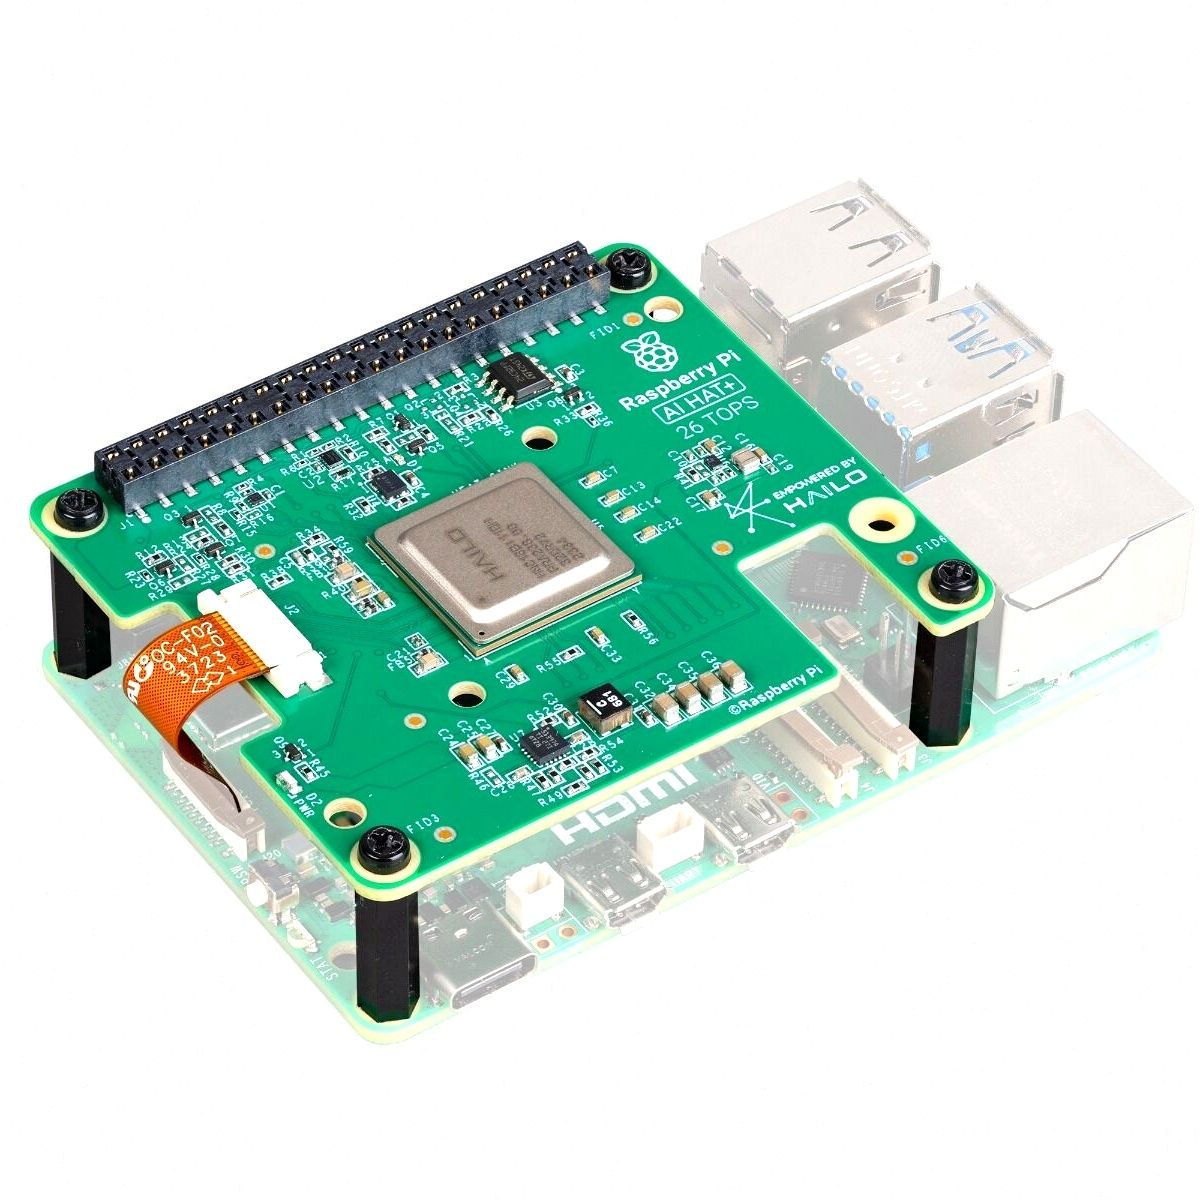
\includegraphics[width=0.75\textwidth]{images/device_with_hailo_processor.jpg}
    \caption{Rozšiřující modul Raspberry Pi AI HAT+ s integrovaným procesorem Hailo-8 (převzato z~\cite{rpishop_ai_hat})}
    \label{fig:hailo_antratek}
\end{figure}
\vspace{-0.2cm}
Řešením tohoto výpočetního omezení je využití specializovaných rozšiřujících desek, jako je modul Raspberry Pi AI HAT+ (znázorněný na obrázku~\ref{fig:hailo_antratek}). Srdcem tohoto modulu, připojeného přes rozhraní \acs{PCIe}, je pokročilý AI procesor Hailo-8 od stejnojmenné izraelské společnosti, jež se specializuje na vývoj výkonných neurálních akcelerátorů.

Klíčovým parametrem tohoto akcelerátoru je deklarovaný výpočetní výkon 26 TOPS (z angl. \textit{Tera Operations Per Second}). Předpona „Tera“ v matematickém vyjádření představuje hodnotu $10^{12}$. Tento čip je tedy fyzicky schopen odbavit masivních $26 \times 10^{12}$ (26 bilionů) operací za jedinou sekundu při inferenci modelu. To, jakým způsobem tohoto výkonu dosahuje, je však stejně důležité jako samotná číselná hodnota. Čipy Hailo využívají inovativní architekturu řízenou datovým tokem (z angl. \textit{Structure-Defined Dataflow Architecture}). Zatímco tradiční \acs{GPU} zpracovávají vrstvy neuronové sítě sekvenčně a neustále zapisují data do externí paměti, Hailo-8 mapuje celou topologii neuronové sítě přímo na své hardwarové zdroje. Obrazová data tak čipem protékají kontinuálně od jedné vrstvy ke druhé bez nutnosti přístupu k externí \acs{RAM}.

Tato obrovská výpočetní propustnost spojená s extrémní energetickou účinností neposkytuje pouze dostatek výkonu pro plynulý běh pokročilých modelů rodiny YOLO. Systému dodává takovou kapacitní rezervu, že dokáže inferenci vysoce paralelizovat. V praxi to znamená, že systém může přijímat a vyhodnocovat obrazová data z několika nezávislých video streamů zcela naráz (například synchronní analýza \acs{RTSP} toků ze dvou různých IP kamer na křižovatce), aniž by došlo k degradaci počtu zpracovaných snímků za sekundu \acs{FPS}~\cite{hailo_alpr_2024, hailo_architecture_2026}. Tím se toto kompaktní hardwarové řešení stává vysoce škálovatelným nástrojem pro robustní a přesné sledování dopravy.

\section{Metodika testování a evaluace}
Vyhodnocení kvality systémů pro detekci, sledování a počítání objektů představuje nedílnou součást návrhu a implementace řešení založených na počítačovém vidění. Cílem evaluace je objektivně posoudit spolehlivost navrženého systému a identifikovat jeho limity. V oblasti dopravního monitorování je však důležité rozlišovat mezi hodnocením samotného matematického modelu (zda správně detekuje obdélníky v izolovaném snímku) a hodnocením systému jako funkčního celku (zda spolehlivě počítá vozidla v čase)~\cite{szeliski_computer_vision, zhou_traffic_survey_2024}.

\subsection{Metodika vyhodnocení detekce v reálném prostředí}
Pro vyhodnocení toho, jak dobře nasazený model YOLO rozeznává objekty v konkrétním kamerovém streamu, je využita metoda manuální obrazové analýzy vybraných referenčních snímků. Vzhledem k absenci předem připraveného a anotovaného datasetu pro danou lokaci jsou z videozáznamu extrahovány reprezentativní statické snímky (např. v různých světelných podmínkách či při různé hustotě provozu).

V těchto izolovaných snímcích je následně provedeno pečlivé manuální sečtení a označení všech reálně přítomných vozidel lidským pozorovatelem, čímž vzniká lokální referenční vzorek (\textit{ground truth}). Výstup detekčního modelu na stejném snímku je s tímto vzorkem vizuálně porovnán, přičemž jsou pro každou třídu identifikovány a zaznamenány následující hodnoty:
\begin{itemize}
    \item \textbf{True Positives (TP):} Správně detekovaná vozidla. Model označil ohraničujícím boxem vozidlo tam, kde se skutečně fyzicky nachází.
    \item \textbf{False Positives (FP):} Falešné detekce. Model označil za vozidlo něco, co ním není (např. stín, značku, sloup), případně vytvořil duplicitní překrývající se detekci pro jedno a to samé auto.
    \item \textbf{False Negatives (FN):} Nerozpoznaná vozidla. Vozidlo na snímku prokazatelně je, ale model jej vůbec nedetekoval.
    \item \textbf{True Negatives (TN):} Správně zamítnuté pozadí. Tento stav označuje prázdný prostor, který model správně ignoroval. V kontextu detekce objektů ohraničujícími boxy se však hodnota TN v praxi nepočítá. 
\end{itemize}

Vztah mezi predikcí modelu a skutečností se ve strojovém učení standardně vizualizuje pomocí tzv. matice záměn (z angl. \textit{Confusion Matrix}), která je pro přehlednost znázorněna v tabulce~\ref{tab:confusion_matrix}.

\begin{table}[H]
    \centering
    \begin{tabular}{|l|l|l|}
        \hline
        \textbf{Predikce/Skutečnost} & \textbf{Vozidlo je přítomno} & \textbf{Vozidlo není přítomno} \\ \hline
        \textbf{Model hlásí detekci} & TP & FP \\ \hline
        \textbf{Model nehlásí detekci} & FN & TN \\ \hline
    \end{tabular}
    \caption{Základní matice záměn (Confusion Matrix).}
    \label{tab:confusion_matrix}
\end{table}

Na základě těchto hodnot jsou následně vypočítány reálné metriky pro danou scénu. Tato analýza poskytuje kritický vhled do toho, do jaké míry případné chyby ve finálním sčítání pocházejí z nepřesné primární detekce a do jaké míry jsou způsobeny až selháním sledovacího algoritmu.

\subsection{Metriky hodnocení detekčních modelů}
Při samotném vývoji a trénování detekčních modelů se k objektivnímu měření výkonu na referenčních datasetech (tzv. \textit{ground truth}) využívá standardizovaná sada matematických metrik~\cite{szeliski_computer_vision}:

\begin{itemize}
    \item \textbf{Precision (Přesnost):} Vyjadřuje podíl skutečně správných detekcí vůči všem detekcím, které model vyprodukoval. Indikuje, jak moc lze věřit modelu, když ohlásí nález vozidla.
    $$ Precision = \frac{TP}{TP + FP} $$
    \item \textbf{Recall (Úplnost):} Udává schopnost systému nalézt všechny relevantní objekty přítomné ve scéně. Definuje se jako podíl správně detekovaných objektů vůči reálnému počtu existujících objektů.
    $$ Recall = \frac{TP}{TP + FN} $$
    \item \textbf{IoU (Intersection over Union):} Vyjadřuje exaktní míru geometrického překryvu mezi predikovaným ohraničujícím boxem ($B_{pred}$) a reálným boxem ($B_{gt}$). Čím více se hodnota blíží k jedné, tím je lokalizace přesnější.
    $$ IoU = \frac{\text{Plocha průniku}}{\text{Plocha sjednocení}} = \frac{|B_{pred} \cap B_{gt}|}{|B_{pred} \cup B_{gt}|} $$
    \item \textbf{mAP (Mean Average Precision):} Představuje komplexní ukazatel výkonu modelu napříč všemi detekovanými třídami ($N$), který zohledňuje přesnost, úplnost i kvalitu lokalizace zjištěnou pomocí křivky Average Precision ($AP$).
    $$ mAP = \frac{1}{N} \sum_{i=1}^{N} AP_i $$
    \item \textbf{Accuracy (Přesnost klasifikace):} Metrika vyjadřující celkový podíl všech správných rozhodnutí. Jak již bylo zmíněno, v detekci objektů má vzhledem k obrovské nerovnováze mezi počtem objektů a plochou prázdného pozadí (obrovské a nedefinovatelné množství TN) jen mizivou vypovídající hodnotu.
    $$ Accuracy = \frac{TP + TN}{TP + TN + FP + FN} $$
\end{itemize}

Vzhledem k tomu, že v rámci této bakalářské práce je implementován a nasazován již hotový, předtrénovaný model z rodiny YOLO, není primárním cílem optimalizace jeho interních vah pomocí výše zmíněných metrik na testovacích datasetech. Cílem je naopak ověření jeho reálné propustnosti a praktické výkonnosti jakožto sčítacího softwarového uzlu v konkrétním dopravním prostředí.

\subsection{Metodika vyhodnocení počítání v reálném prostředí}
Vyhodnocení správnosti sčítání objektů je v dopravních aplikacích klíčové. Na rozdíl od detekce izolovaných snímků se zde hodnotí konzistence sledovacího algoritmu (např. zda udrží ID vozidla) a správná prostorová identifikace průjezdů vyhrazenými počítacími liniemi. 

Hlavními zdroji chyb v reálném prostředí jsou časté vizuální překryvy objektů (okluze), ztráta identifikátoru způsobující opakované započítání téhož vozidla, nebo dynamické změny světelných podmínek a vrhání stínů. Jak potvrzují srovnávací studie zaměřené na reálné nasazení video-detekčních počítacích systémů, právě tyto faktory vnějšího prostředí představují největší výzvu pro udržení vysoké a stabilní provozní přesnosti~\cite{zhou_traffic_survey_2024}, \cite{pronello_2023}.

V reálném nasazení bez existence předem připravených exaktních datových sad je standardní evaluační metodou vytvoření vlastní sady referenčních dat (tzv. ground truth) formou nezávislého manuálního sčítání z pořízeného videozáznamu~\cite{mdpi_roi_tracking_2022}, \cite{pronello_2023}. Referenční hodnota je tak získána nezávislým pozorováním, čímž je stanoven skutečný počet průjezdů vozidel ($N_{real}$). Tento údaj je následně porovnán s počtem vozidel detekovaných automatizovaným systémem ($N_{sys}$) pomocí metriky poměrové přesnosti sčítání ($Accuracy_{count}$):

$$Accuracy_{count} = \left( 1 - \frac{|N_{real} - N_{sys}|}{N_{real}} \right) \cdot 100 \ [\%]$$

Tato metrika věrně a zcela exaktně reflektuje celkovou provozní úspěšnost systému při kontinuálním sčítání vozidel, a právě ona bude využita jako primární hodnoticí ukazatel v testovací části této práce.

\section{Etické aspekty a GDPR}
Při návrhu, nasazení a provozu jakýchkoliv kamerových systémů na veřejných prostranstvích a dopravních komunikacích je absolutně nezbytné zohlednit principy ochrany osobních údajů. Tyto povinnosti primárně vyplývají z platného Nařízení Evropského parlamentu a Rady (EU) 2016/679, obecně známého pod zkratkou \acs{GDPR} (z angl. \textit{\acl{GDPR}})\acused{GDPR}. Moderní kamerové systémy totiž ze své podstaty mohou neúmyslně zachytávat citlivé identifikační prvky, jakými jsou tváře chodců, řidičů nebo konkrétní registrační značky vozidel.

Navrhované řešení v rámci této bakalářské práce proto plně a striktně respektuje moderní přístup tzv. \textit{Privacy by Design} (ochrana soukromí již od fáze samotného návrhu softwarové architektury). Tohoto principu je dosaženo právě díky integraci konceptu Edge AI. Veškeré algoritmické zpracování obrazových dat z kamery probíhá plně lokálně, přímo v operační paměti okrajového zařízení, které je umístěno bezprostředně u zdroje videa~\cite{li_edge_ai_2020}. 

Díky lokální a okamžité inferenci se žádný surový obrazový signál, videozáznam ani snímky obsahující potenciální osobní údaje nikam neukládají, neodesílají se přes nezabezpečené sítě a nejsou nahrávány do žádného vzdáleného cloudového úložiště. Do databázového systému se propisují a k následné vizualizaci odesílají pouze finální, přísně anonymizovaná a agregovaná numerická metadata – například celkový typ objektu (automobil, chodec), hrubý časový údaj, směr jeho pohybu a identifikátor sčítací brány. 

Tento architektonický přístup bezezbytku naplňuje zásadu minimalizace osobních údajů, která je jedním z nosných a nejdůležitějších pilířů legislativy GDPR. Systém tak poskytuje plnohodnotná statistická data pro analýzu dopravy, aniž by jakýmkoliv způsobem zasahoval do soukromí účastníků provozu.

\chapter{Návrh systému}
\section{Požadavky na systém}
Navrhovaný systém je určen pro automatizovanou analýzu silniční dopravy 
pomocí metod počítačového vidění. Cílem je detekce a sledování vozidel 
v reálném čase a následná extrakce statistických údajů o jejich průjezdech.

Mezi hlavní funkční požadavky patří:

\begin{itemize}
    \item detekce vozidel v obrazové sekvenci,
    \item klasifikace detekovaných vozidel do kategorií,
    \item sledování klasifikovaných objektů napříč jednotlivými snímky,
    \item identifikace průjezdu klasifikovaných objektů definovanou detekční linií (ROI),
    \item ukládání detekčních událostí do databáze,
    \item vizualizace agregovaných statistik.
\end{itemize}

Systém musí být schopen provozu v reálném čase na vestavěném zařízení s omezenými výpočetními prostředky. Z tohoto důvodu je navržena architektura založená na principu \textit{edge computing}, kdy je inference neuronové sítě prováděna přímo na zařízení v místě sběru dat~\cite{akira_edge_cloud}.

\section{Celková architektura a tok dat}

%Architektura systému je navržena jako vícevrstvá a modulární. 
%Jednotlivé komponenty jsou odděleny podle své funkce, což umožňuje lepší škálovatelnost, robustnost a údržbu systému.


Architektura systému je navržena jako vícevrstvá, distribuovaná a modulární. Jednotlivé komponenty jsou odděleny podle své funkce a komunikují spolu asynchronně prostřednictvím lehkého zprávového protokolu MQTT~\cite{mqtt_oasis_2019}. Toto rozdělení umožňuje lepší škálovatelnost, robustnost a minimalizaci vzájemné závislosti komponent, což plně odpovídá moderním architekturám dopravních monitorovacích systémů založených na počítačovém vidění~\cite{zhou_traffic_survey_2024}.

\begin{figure}[H]
    \centering
    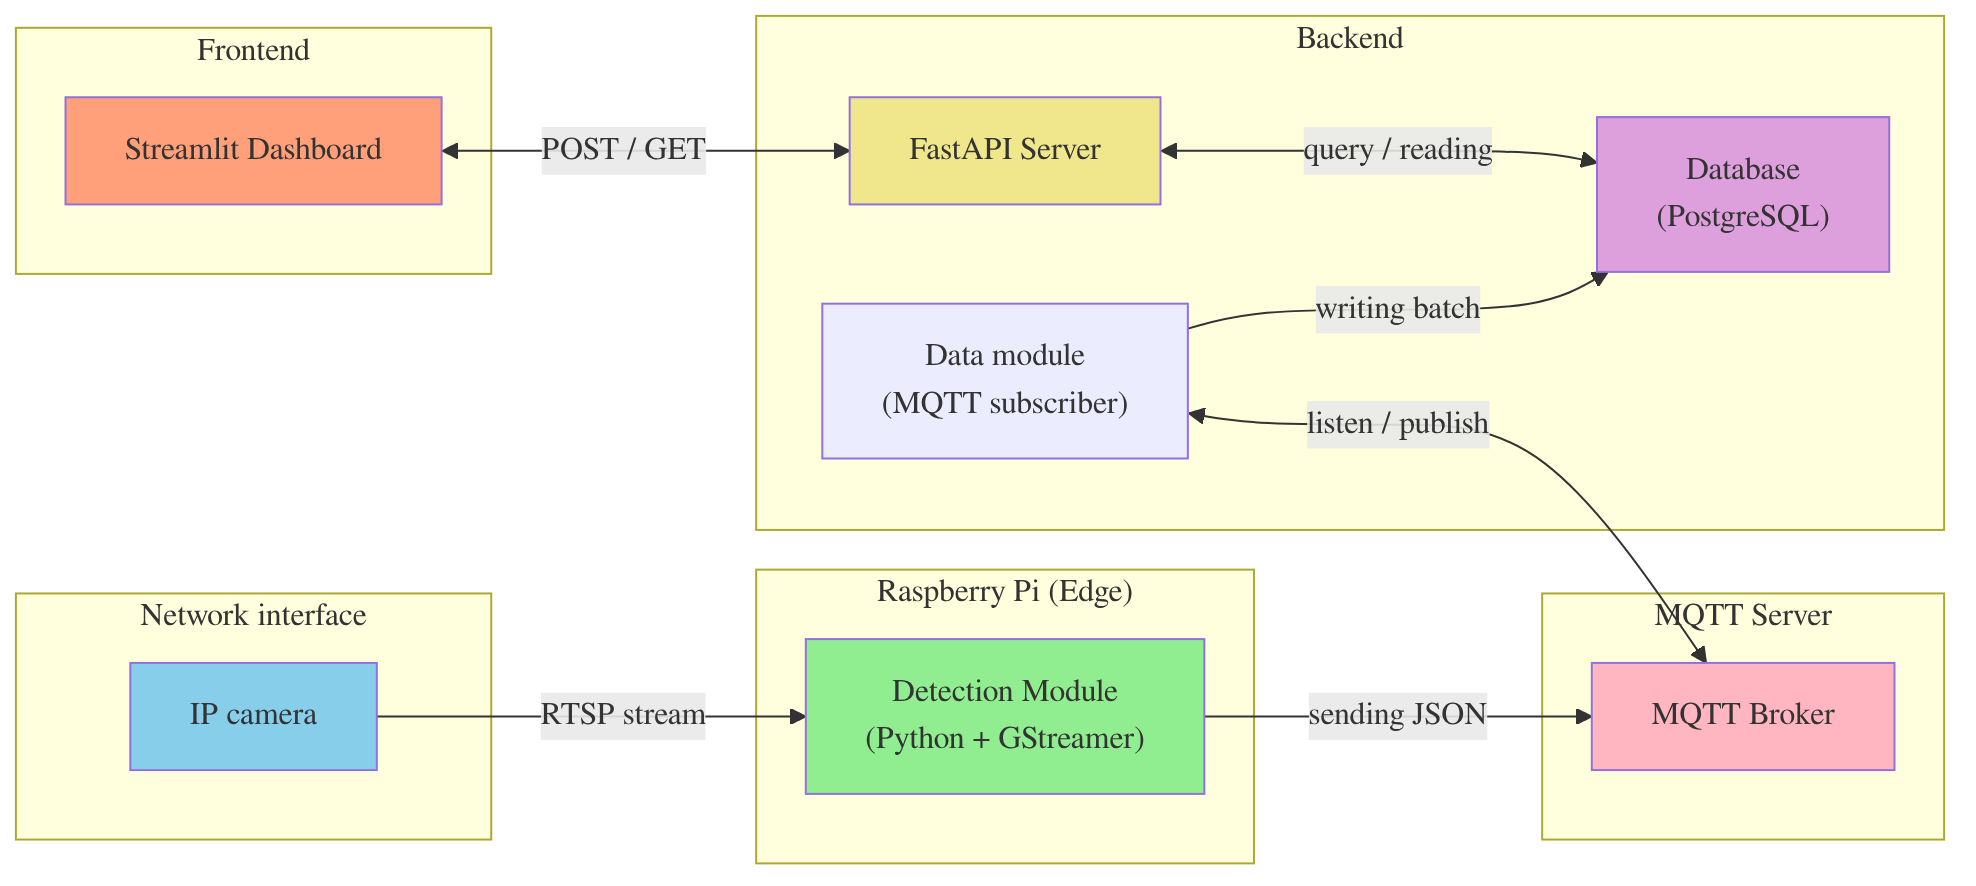
\includegraphics[width=\textwidth]{images/architecture.png}
    \caption{Navržená architektura systému pro analýzu dopravy}
    \label{fig:architektura}
\end{figure}

Na obrázku~\ref{fig:architektura} je znázorněna celková topologie navrženého řešení. Systém je rozdělen do pěti funkčních vrstev, kterými postupně prochází tok dat:

\begin{enumerate}
    \item \textbf{Vrstva akvizice obrazu (Síťová vrstva):} Koncová IP kamera poskytuje kontinuální video stream přenášený po lokální síti pomocí protokolu \acs{RTSP}.
    \item \textbf{Vrstva zpracování videa (Edge vrstva):} Zde se provádí detekce, klasifikace a sledování objektů pomocí AI modulu. Obrazová data jsou přijata na okrajovém zařízení, předzpracována a předána detekčnímu modelu typu YOLO~\cite{redmon_yolo_2016}, který provádí detekci a klasifikaci objektů. Následný sledovací algoritmus (např. na principu SORT~\cite{SORT_original_2016}) přiřazuje jednotlivým objektům unikátní identifikátory a vyhodnocuje jejich průchod přes virtuální detekční linii~\cite{mdpi_roi_tracking_2022}.
    \item \textbf{Komunikační vrstva:} Vygenerované strukturované události o průjezdech jsou asynchronně odesílány prostřednictvím MQTT brokeru~\cite{mqtt_oasis_2019} do datové vrstvy.
    \item \textbf{Datová a backendová vrstva:} Zajišťuje trvalé ukládání přijatých událostí do relační databáze a poskytuje aplikační rozhraní (REST API) pro přístup k těmto datům.
    \item \textbf{Aplikační a vizualizační vrstva (Frontend):} Komunikuje s backendem pomocí REST API a zprostředkovává agregované statistické přehledy koncovému uživateli.
\end{enumerate}

Oddělení jednotlivých kroků do samostatných vrstev umožňuje vysokou modularitu systému a minimalizaci vzájemné závislosti komponent.

\section{Výběr hardwaru}
Pro zajištění spolehlivého chodu celého řešení je hardwarová část fyzicky rozdělena na prvek pro sběr obrazových dat a výpočetní uzel pro jejich zpracování.

\textbf{Kamerový systém:} Pro dosažení dostatečné kvality detekce je využita IP kamera značky Hikvision, která umožňuje síťový přenos video streamu prostřednictvím protokolů \acs{RTSP} nebo \acs{HTTP} (z angl. \textit{\acl{HTTP}})\acused{HTTP}. Použití IP kamery dovoluje flexibilní umístění zařízení mimo samotný výpočetní uzel a současně poskytuje vyšší odolnost vůči povětrnostním podmínkám v porovnání s běžnými kamerovými moduly pro vestavěná zařízení. %Kamera poskytuje obraz ve vysokém rozlišení, což je klíčové pro přesnou detekci vozidel zejména ve větší vzdálenosti od kamery.

\textbf{Zpracovatelská jednotka:} Jako výpočetní platforma na hraně sítě (edge zařízení), která přijímá datový tok z lokální sítě, je navrženo zařízení Raspberry Pi 5. Tato platforma představuje vhodný kompromis mezi výkonem, spotřebou a pořizovací cenou~\cite{raspberrypi_docs_2024}. Pro zajištění real-time inference neuronové sítě je doplněna o dedikovaný AI akcelerátor Hailo-8 kompatibilní s touto platformou~\cite{raspberrypi_ai_kit}. Tento přístup umožňuje efektivní zpracování obrazu přímo na místě bez nutnosti využití cloudových služeb.

\section{Návrh softwarových modulů}
%Softwarová architektura je navržena jako distribuovaná a asynchronní. Jednotlivé komponenty komunikují prostřednictvím lehkého zprávového protokolu MQTT \cite{mqtt_oasis_2019}.

\subsection{Objektový návrh aplikace (UML)}
Pro zajištění modularity, snadné testovatelnosti a budoucí rozšiřitelnosti byl softwarový kód systému navržen s využitím objektově orientovaného programování (OOP). Jednotlivé funkční celky od zpracování videa přes mezivrstvu pro přenos zpráv až po databázové operace a aplikační rozhraní, jsou zapouzdřeny do samostatných tříd a modulů (viz obrázek~\ref{fig:class_diagram}). Tento přístup umožňuje provozovat detekční část zcela autonomně z příkazové řádky, nebo ji dynamicky řídit prostřednictvím webového rozhraní.

\begin{figure}[H]
    \centering
    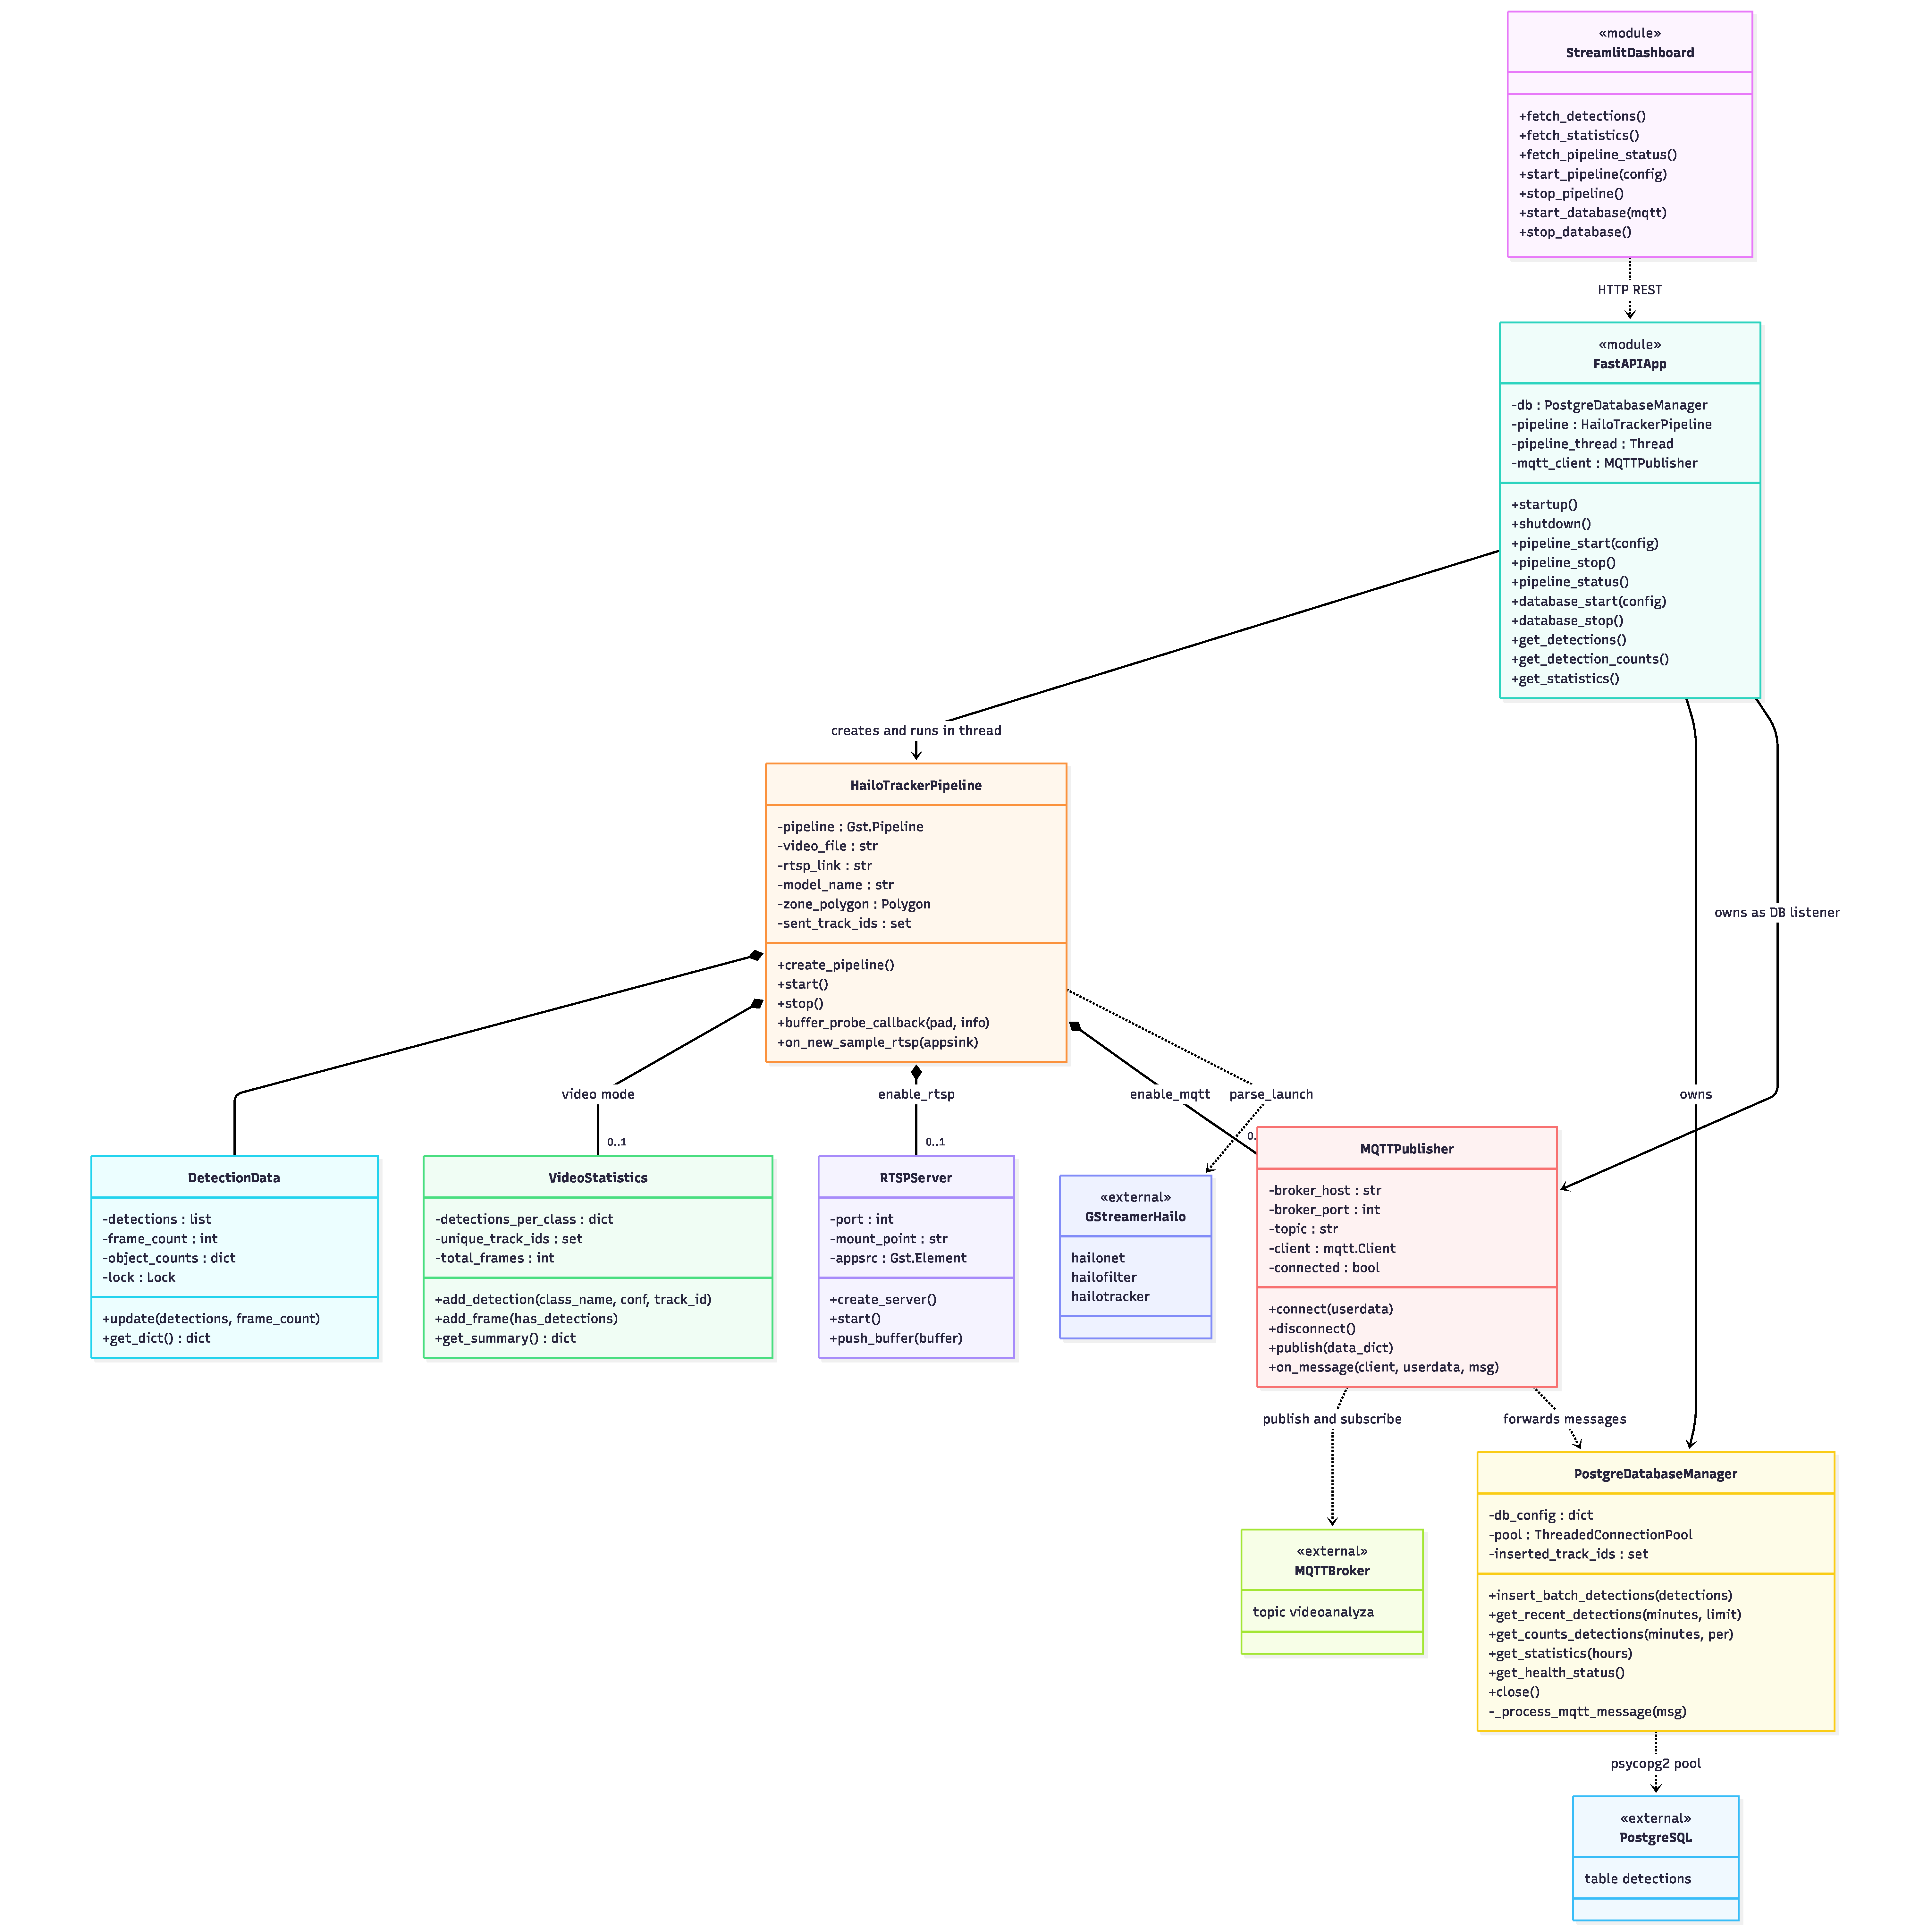
\includegraphics[
        page=1,    
    width=1\textwidth
    ]{images/System_UML.pdf}
    \caption{UML diagram tříd navrženého dopravního monitorovacího systému.}
    \label{fig:class_diagram}
\end{figure}

Struktura softwarové aplikace se skládá z následujících klíčových tříd a modulů:
\begin{itemize}
    \item \textbf{\texttt{HailoTrackerPipeline}} – Ústřední třída detekčního modulu na hraně sítě. Zapouzdřuje sestavení a řízení multimediálního řetězce (\texttt{Gst.Pipeline}), komunikaci s akcelerátorem Hailo-8 a registraci zpětného volání (\texttt{buffer\_probe\_callback}). Současně udržuje geometrickou definici oblasti zájmu (\texttt{zone\_polygon}) a množinu již odeslaných identifikátorů (\texttt{sent\_track\_ids}) pro eliminaci duplicit.
    \item \textbf{\texttt{DetectionData}} – Datová struktura zajišťující vláknově bezpečné (\textit{thread-safe}) uchovávání aktuálních výsledků detekce a počtů objektů pomocí synchronizačního zámku (\texttt{Lock}). Poskytuje metody pro serializaci dat do slovníku a generování překryvného textu do obrazu.
    \item \textbf{\texttt{VideoStatistics}} a \textbf{\texttt{RTSPServer}} – Volitelné (kompozičně vázané) pomocné třídy. \texttt{VideoStatistics} slouží k agregaci souhrnných metrik při zpracování video souborů, zatímco \texttt{RTSPServer} umožňuje prostřednictvím prvku \texttt{appsrc} přeposílat zpracovaný video stream s vykreslenými detekcemi dále do sítě.
    \item \textbf{\texttt{MQTTPublisher}} – Univerzální komunikační třída zapouzdřující klienta protokolu MQTT. V architektuře plní dvojí roli: na straně detekční pipeline zajišťuje publikaci dat (\texttt{publish}) do tématu \texttt{videoanalyza}, zatímco na straně serveru funguje jako odběratel (\textit{listener}), který přijaté zprávy předává metodě \texttt{on\_message} ke zpracování do databáze.
    \item \textbf{\texttt{PostgreDatabaseManager}} – Třída zodpovědná za perzistenci a čtení dat z relační databáze PostgreSQL. Využívá fond spojení (\texttt{ThreadedConnectionPool}) z knihovny \texttt{psycopg2}, zpracovává příchozí MQTT zprávy, provádí dávkové vkládání záznamů (\texttt{insert\_batch\_detections}) a poskytuje agregační metody pro analytické dotazy.
    \item \textbf{\texttt{FastAPIApp}} a \textbf{\texttt{StreamlitDashboard}} – Aplikační a prezentační moduly. Modul \texttt{FastAPIApp} poskytuje REST API rozhraní pro čtení statistik z databáze a zároveň umožňuje vzdáleně spouštět a zastavovat detekční pipeline v samostatném vlákně (\texttt{Thread}). Modul \texttt{StreamlitDashboard} s tímto rozhraním komunikuje přes protokol HTTP a zajišťuje interaktivní vizualizaci dat pro koncového uživatele.
\end{itemize}

\subsection{Detekční modul a logika počítání (ROI)}
Detekční modul je založen na konvoluční neuronové síti typu YOLO, která umožňuje rychlou lokalizaci a klasifikaci objektů v obraze~\cite{redmon_yolo_2016}. Pro následné sledování těchto objektů napříč snímky je navržen algoritmus typu SORT~\cite{SORT_original_2016}, případně jeho rozšířená varianta DeepSORT~\cite{wojke_deepsort_2017}. Každému sledovanému objektu je tak přiřazen unikátní identifikátor (ID), jenž je udržován po celou dobu jeho výskytu ve scéně.

\textbf{Logika detekční zóny (ROI):}
Pro účely filtrace a počítání relevantních vozidel je v obraze definována virtuální oblast zájmu (tzv. \textit{Region of Interest} - ROI) ve tvaru obecného polygonu~\cite{mdpi_roi_tracking_2022}. Polygonální reprezentace umožňuje přesně vymezit sledovaný jízdní pruh a odfiltrovat nežádoucí detekce mimo komunikaci. Započítání vozidla proběhne v okamžiku, kdy se geometrický střed jeho ohraničujícího rámečku (\textit{bounding box}) ocitne uvnitř definovaného polygonu. Aby nedocházelo k vícenásobnému započítání téhož vozidla v kolejnych snímcích, systém udržuje evidenci již zpracovaných identifikátorů \texttt{track\_id} a každé vozidlo odešle ke zpracování pouze jednou.

\subsection{Ukládání dat, databázové schéma a vizualizace}
Strukturované detekční události jsou ukládány do relační databáze PostgreSQL, která umožňuje spolehlivé uchování dat a jejich následné statistické vyhodnocení~\cite{psycopg_docs_2025}. Pro účely trvalé evidence byla navržena primární tabulka \texttt{detections}, jejíž struktura je popsána v tabulce~\ref{fig:erd}. Každý zaznamenaný průjezd vozidla přes detekční linii vygeneruje právě jeden záznam.

\subsubsection{Datový model}
Datový model je založen na hlavní entitě \textit{detections} (znázorněné na obrázku~\ref{fig:erd}), která uchovává informace o jednotlivých detekcích a průjezdech vozidel. Struktura tabulky je navržena s ohledem na vysoký objem dat a efektivní časové dotazování.

\begin{figure}[H]
    \centering
    % page=1 vybere první stránku
    % trim={vlevo dole vpravo nahoře} ořízne okraje (hodnoty si případně dolaď)
    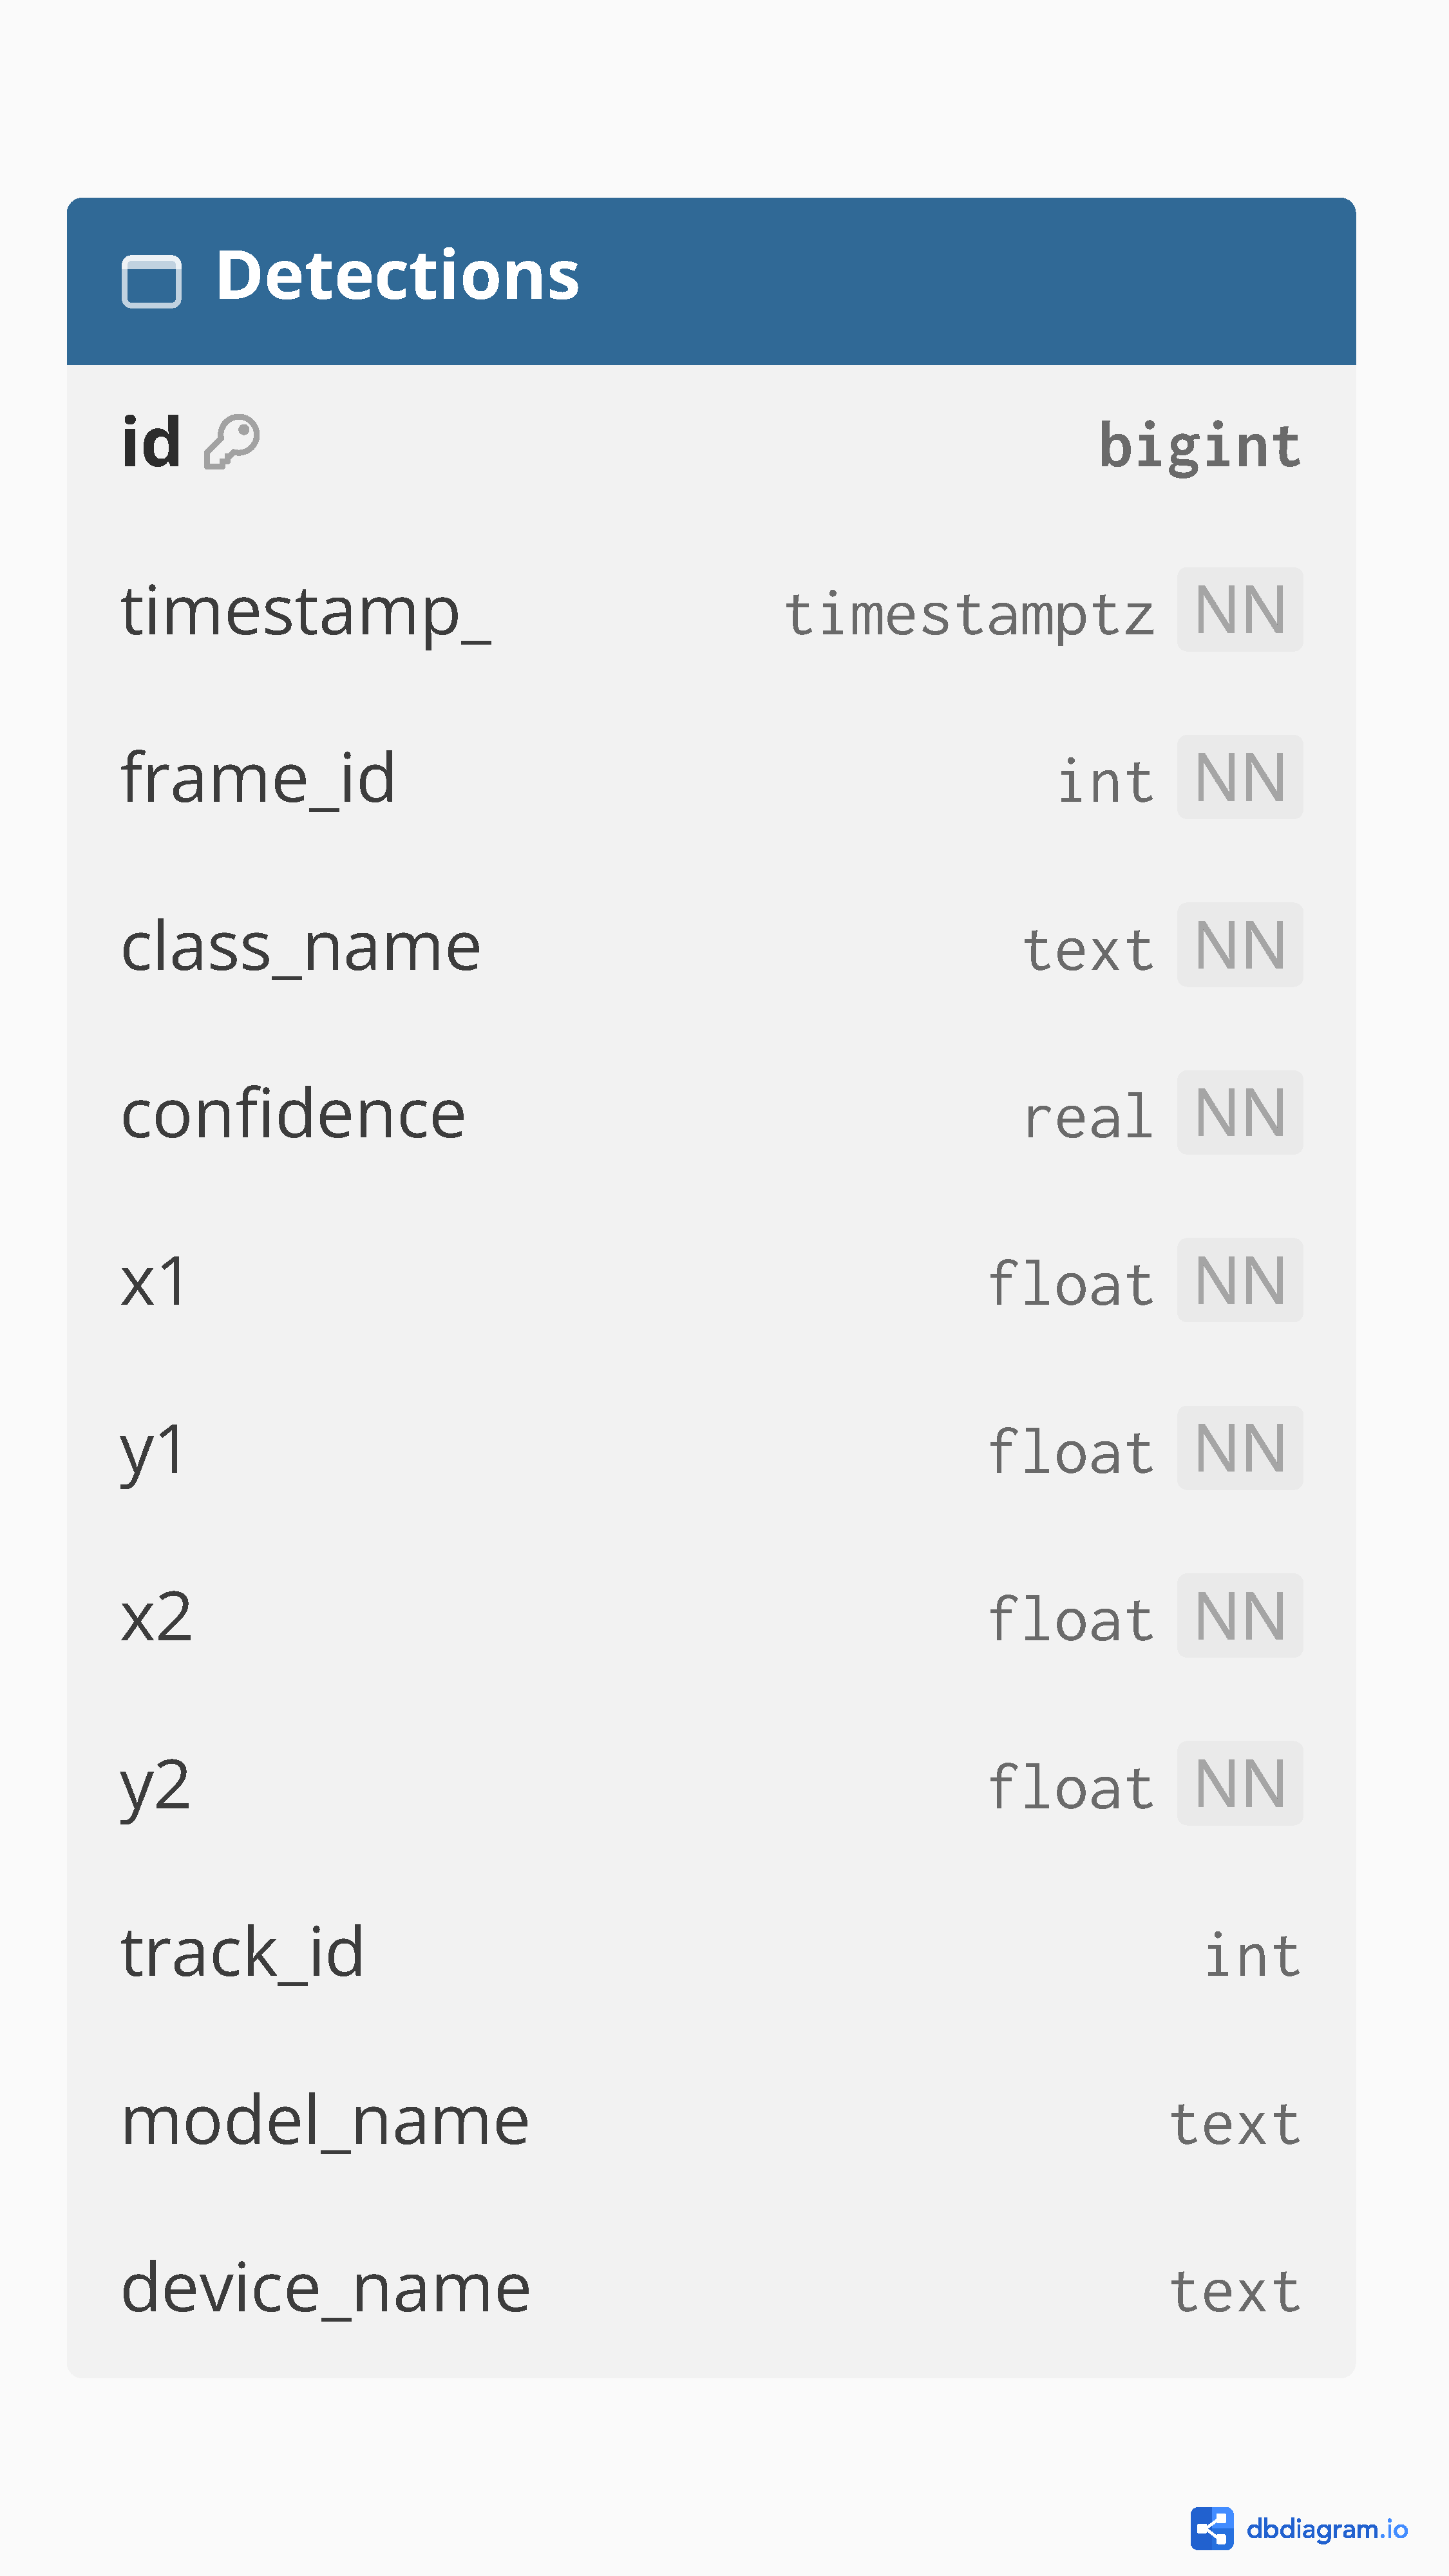
\includegraphics[
        page=1,
        trim={2cm 5cm 2cm 5cm},
        clip,
        width=0.35\textwidth
    ]{images/DB_diagram.pdf}
    \caption{ER diagram databázového modelu.}
    \label{fig:erd}
\end{figure}

\paragraph{Popis atributů tabulky \textit{detections}:}
\begin{itemize}
    \item \textbf{id (BIGSERIAL)} – Primární klíč tabulky. Automaticky generovaná unikátní hodnota sloužící k jednoznačné identifikaci každé detekce. Typ \textit{BIGSERIAL} byl zvolen s ohledem na předpokládaný vysoký objem záznamů.
    \item \textbf{timestamp\_ (TIMESTAMPTZ)} – Čas detekce objektu. Datový typ \textit{TIMESTAMPTZ} umožňuje ukládání časové informace včetně časové zóny, což je důležité pro přesnou časovou analýzu dopravních událostí.
    \item \textbf{frame\_id (INTEGER)} – Identifikátor snímku, ve kterém byla detekce provedena. Umožňuje zpětné dohledání konkrétního snímku v případě analýzy nebo ladění systému.
    \item \textbf{class\_name (TEXT)} – Název detekované třídy objektu (např. \textit{car}, \textit{truck}, \textit{bus}). Tento atribut umožňuje následnou agregaci a statistické vyhodnocení podle typu vozidla.
    \item \textbf{confidence (REAL)} – Pravděpodobnost detekce generovaná neuronovou sítí. Je definováno omezení \texttt{CHECK (confidence >= 0 AND confidence <= 1)}, které zajišťuje validitu ukládaných hodnot.
    \item \textbf{x1, y1, x2, y2 (FLOAT)} – Souřadnice ohraničujícího obdélníku (\textit{bounding box}) detekovaného objektu. Hodnoty představují levý horní a pravý dolní roh objektu v rámci zpracovávaného obrazu. Integritní omezení \texttt{CHECK (x2 > x1 AND y2 > y1)} zajišťuje geometrickou konzistenci dat.
    \item \textbf{track\_id (INT)} – Identifikátor sledovaného objektu, generovaný sledovacím algoritmem. Umožňuje sledování pohybu konkrétního vozidla napříč více snímky.
    \item \textbf{model\_name (TEXT)} – Označení použitého detekčního modelu (např. \textit{yolov8s}). Sloupec je navržen pro potřeby budoucího porovnávání úspěšnosti různých verzí neuronových sítí nad reálnými daty.
    \item \textbf{device\_name (TEXT)} – Identifikátor konkrétní výpočetní jednotky (edge zařízení) nebo kamery. Zajišťuje připravenost databázového schématu na horizontální škálování systému do více lokalit.
\end{itemize}

\textbf{Indexování:} S ohledem na charakter dotazů byly vytvořeny indexy nad atributy \textit{timestamp\_}, \textit{class\_name} a \textit{track\_id}. Tyto indexy optimalizují zejména dotazy na poslední detekce, časově omezené statistiky, filtrování podle typu vozidla a analýzu pohybu konkrétního objektu. Použití sestupného indexu nad atributem \textit{timestamp\_} umožňuje efektivní získávání nejnovějších detekcí, což je častý scénář v reálném provozu systému.

\subsubsection{Analýza a vizualizace dat}
Backendová vrstva zpřístupňuje uložená data prostřednictvím REST API postaveného na moderním frameworku FastAPI. Pro následné numerické transformace a časové agregace záznamů systém využívá knihovny NumPy~\cite{harris_numpy_2020} a Pandas~\cite{mckinney_pandas_2010}. Koncové webové rozhraní s interaktivními grafy je navrženo s využitím frameworku Streamlit v kombinaci s grafickou knihovnou Plotly~\cite{plotly_docs_2015}, což umožňuje interaktivní zobrazení časových řad, histogramů a agregovaných statistik dopravního provozu.

\subsection{Technologie}
Celkový přehled zvolených technologií pro jednotlivé vrstvy navržené architektury shrnuje tabulka~\ref{tab:tech_stack}.

\begin{table}[H]
    \centering
    \renewcommand{\arraystretch}{1.2}
    \begin{tabular}{|l|l|}
        \hline
        \textbf{Komponenta systému} & \textbf{Zvolená technologie} \\ \hline
        Operační systém (Edge) & Raspberry Pi OS (Debian Linux) \\ \hline
        Programovací jazyk & Python 3.11 \\ \hline
        Zpracování videa & GStreamer \\ \hline
        AI inference a sledování & HailoRT + TAPPAS (YOLO) \\ \hline
        Komunikační protokol & MQTT \\ \hline
        Databázové úložiště & PostgreSQL + Psycopg \\ \hline
        Backend a REST API & FastAPI + Pandas / NumPy \\ \hline
        Vizualizační frontend & Streamlit + Plotly \\ \hline
    \end{tabular}
    \caption{Přehled technologického stacku navrženého systému.}
    \label{tab:tech_stack}
\end{table}

Výhodou využití frameworku GStreamer je především jeho vysoký výkon a efektivní práce s daty, protože většina jeho pluginů je implementována v jazyce C/C++. Díky tomu může být video stream zpracováván s minimální režijní vrstvou a bez nutnosti přenosu dat mezi interpretem Pythonu a nativním kódem. Jednotlivé prvky pipeline navíc mohou běžet paralelně, což umožňuje efektivní využití systémových prostředků a dosažení vyššího výkonu při zpracování video streamu v reálném čase.


\chapter{Implementace systému}
\section{Konfigurace prostředí a automatizace běhu}
Pro praktickou realizaci systému na cílové platformě Raspberry Pi~5 byl nainstalován operační systém Raspberry Pi OS (založený na distribuci Debian Linux)~\cite{raspberrypi_docs_2024}, který poskytuje plnou podporu hardwarových rozhraní, dostupnost potřebných knihoven pro práci s obrazem a sítí a kompatibilitu s ovladači AI akcelerátoru Hailo-8. Řídicí skripty byly implementovány v jazyce Python~3.11~\cite{python_docs_313_2025}.
%Implementace systému byla realizována v programovacím jazyce Python ve verzi 3.11 \cite{python_docs_313_2025}. 
%Python byl zvolen zejména díky:
%\begin{itemize}
%    \item široké podpoře knihoven pro počítačové vidění,
%    \item jednoduché integraci s databázovými systémy,
%    \item dostupnosti frameworků pro tvorbu webového API.
%\end{itemize}

\subsection{Automatická instalace závislostí a spouštění služeb}
Pro zajištění plné reprodukovatelnosti prostředí a snadného nasazení na nové zařízení byl vytvořen instalační skript, který automatizuje přípravu celého systému. Tento skript provádí:
\begin{itemize}
    \item instalaci systémových balíčků a multimediálního frameworku GStreamer,
    \item instalaci běhového prostředí HailoRT a knihoven TAPPAS~\cite{tappas_user_guide_331} pro AI akcelerátor,
    \item vytvoření virtuálního prostředí a instalaci Python knihoven (Ultralytics, Shapely, Paho-MQTT, Psycopg, FastAPI, Streamlit, Pandas, Plotly),
    \item nastavení systémových oprávnění a proměnných prostředí.
\end{itemize}

Aby byl zajištěn plně autonomní provoz systému v reálných podmínkách (např. při výpadku napájení a následném restartu zařízení), byl v operačním systému nakonfigurován spouštěcí mechanismus automatického spuštění hlavních služeb. Po inicializaci operačního systému spouštěcí skript nastaví potřebné proměnné prostředí a ve správném pořadí automaticky odstartuje hlavní komponenty:
\begin{enumerate}
    \item detekční pipeline běžící na edge zařízení,
    \item odběratelskou službu (MQTT subscriber) zajišťující zápis do databáze,
    \item backendový server (FastAPI) a webové vizualizační rozhraní (Streamlit).
\end{enumerate}

Tento přístup umožňuje plně autonomní provoz zařízení bez nutnosti manuálního zásahu po restartu systému. 

\section{Příprava a kompilace detekčního modelu}
\subsection{Volba varianty modelu a předzpracování}
%Pro detekci objektů byl zvolen model architektury YOLO (You Only Look Once), který je navržen pro real-time detekci objektů v jednom průchodu neuronovou sítí \cite{redmon_yolo_2016}. Modely YOLO jsou známé vysokým poměrem mezi přesností a rychlostí inference, což je klíčové pro nasazení na vestavěné edge platformě.

V rámci implementace nebyl model trénován od začátku, ale byl využit předtrénovaný model rodiny YOLOv8 natrénovaný na datasetu COCO~\cite{lin_coco_2014}. Během vývoje byly experimentálně zkompilovány a otestovány varianty YOLOv8n, YOLOv8s a YOLOv8m, které se liší počtem parametrů. Pro finální nasazení byla zvolena varianta \textbf{YOLOv8m}, jež na cílové platformě vykazovala optimální kompromis mezi rychlostí inference a přesností detekce vzdálenějších vozidel.

Pro nasazení modelu na akcelerátor Hailo-8 lze buď využít předpřipravené modely z repozitáře Hailo RPi5 Examples~\cite{hailo_rpi5_examples}, nebo provést vlastní kompilaci do binárního formátu HEF (\textit{Hailo Executable Format}) pomocí nástroje Hailo Dataflow Compiler (DFC)~\cite{hailo_dfc_docs}. V této práci byl realizován kompletní proces vlastní kompilace. Před samotnou inferencí jsou vstupní snímky vždy převzorkovány na rozlišení $640 \times 640$ pixelů a převedeny do barevného formátu RGB.
%Model byl následně optimalizován a zkompilován pro běh na AI akcelerátoru Hailo pomocí nástroje Hailo Dataflow Compiler. Pro ověření funkčnosti modelu byla použita reálná data z dopravní kamery. Testovací sekvence obsahovaly vozidla různých tříd a byly zaznamenány za různých světelných podmínek.

\subsection{Export modelu do formátu ONNX}
Prvním krokem přípravy pro kompilátor Hailo DFC je převod vah modelu z nativního formátu PyTorch (\texttt{.pt}) do standardizovaného meziformátu ONNX (\textit{Open Neural Network Exchange}). Export byl proveden pomocí knihovny Ultralytics s pevně definovanou velikostí vstupu a zjednodušením výpočetního grafu (ukázka~\ref{lst:onnx_export}).

%ONNX představuje standardizovaný formát pro reprezentaci modelů neuronových sítí, který umožňuje interoperabilitu mezi různými frameworky pro strojové učení. Model YOLOv8 byl exportován z knihovny Ultralytics do formátu ONNX s velikostí vstupního obrazu 640×640 pixelů.

\begin{lstlisting}[language=Python, caption={Export modelu YOLOv8m do formátu ONNX.}, label={lst:onnx_export}]
from ultralytics import YOLO

model = YOLO("yolov8m.pt")

model.export(
    format="onnx",
    imgsz=640,
    opset=11,
    simplify=True
)
\end{lstlisting}

Výsledkem tohoto kroku je soubor \texttt{yolov8m.onnx}, který slouží jako přímý vstup pro optimalizační nástroje Hailo.

\subsection{Kvantizace a kompilace do formátu HEF}
Převod ONNX modelu do spustitelného formátu HEF byl proveden pomocí nástroje \texttt{hailomz} z knihovny Hailo Model Zoo~\cite{hailo_model_zoo}. Tento proces zahrnuje čtyři fáze:
\begin{enumerate}
    \item překlad (parsing) ONNX grafu do meziformátu HAR (\textit{Hailo Archive}),
    \item optimalizaci a kvantizaci vah z 32bitové plovoucí řádové čárky (FP32) na 8bitová celá čísla (INT8),
    \item alokaci hardwarových výpočetních zdrojů cílového čipu,
    \item generování finálního binárního souboru HEF.
\end{enumerate}

Pro správné provedení post-tréninkové kvantizace (PTQ) do formátu INT8 vyžaduje kompilátor kalibrační sadu čítající řádově stovky až tisíce snímků, na kterých analyzuje statistické rozložení aktivací v jednotlivých vrstvách. Pro tento účel byla využita validační část datasetu COCO (\texttt{val2017}) obsahující 5\,000 snímků~\cite{lin_coco_2014}. Vzhledem k vysoké výpočetní a paměťové náročnosti procesu kompilace (který trvá v řádu desítek minut) probíhal tento krok na externí pracovní stanici pomocí příkazu uvedeného v ukázce~\ref{lst:hailo_compile}.

\begin{lstlisting}[language=bash, caption={Kompilace modelu YOLOv8m pomocí nástroje Hailo Model Zoo.}, label={lst:hailo_compile}]
hailomz compile yolov8m \
    --hw-arch hailo8 \
    --calib-path ./coco_val2017 \
    --classes 80
\end{lstlisting}

Vygenerovaný soubor \texttt{yolov8m.hef} byl následně přenesen na zařízení Raspberry Pi~5, kde umožňuje provádět inferenci s výrazně nižší latencí a spotřebou energie při zachování vysoké detekční přesnosti.

\section{Implementace zpracování videa a detekce}

\subsection{Konstrukce GStreamer pipeline}
Zpracování obrazového toku v reálném čase je postaveno na zřetězení zásuvných modulů frameworku GStreamer. Pipeline se připojuje k IP kameře přes protokol RTSP, provádí hardwarově či softwarově akcelerované dekódování komprimovaného formátu H.264, škáluje obraz na rozlišení $640 \times 640$ pixelů a předává jej specializovaným prvkům Hailo (ukázka~\ref{lst:gst_pipeline}).

\begin{lstlisting}[language=Python, caption={Zjednodušená konstrukce GStreamer pipeline.}, label={lst:gst_pipeline}]
pipeline_str = (
    "rtspsrc location=rtsp://CAMERA_IP latency=150 "
    "! rtph264depay ! h264parse ! avdec_h264 "
    "! videoconvert ! videoscale "
    "! video/x-raw,width=640,height=640,format=RGB "
    "! hailonet hef-path=yolov8m.hef batch-size=1 "
    "nms-score-threshold=0.6 nms-iou-threshold=0.5 "
    "! hailofilter function-name=yolov8m "
    "! hailotracker iou-thr=0.5 "
    "! videoconvert ! fakesink"
)
\end{lstlisting}

Samotnou inferenci na akcelerátoru zajišťuje prvek \texttt{hailonet}. Parametr \texttt{batch-size=1} garantuje, že každý přijatý snímek je zpracován okamžitě bez čekání na naplnění dávky, což minimalizuje latenci. Parametry \texttt{nms-score-threshold} a \texttt{nms-iou-threshold} konfigurují algoritmus \textit{Non-Maximum Suppression} (NMS), jenž filtruje detekce s nízkou spolehlivostí a odstraňuje vícenásobné překrývající se rámečky nad stejným vozidlem. Následující prvek \texttt{hailofilter} provádí post-processing tenzorů a modul \texttt{hailotracker} přiřazuje objektům sledovací identifikátory na základě překryvu (\texttt{iou-thr=0.5}).

Pro účely ladění nebo paralelního ukládání záznamu lze pipeline na konci rozvětvit pomocí prvku \texttt{tee}, který duplikuje datový tok do více nezávislých větví (ukázka~\ref{lst:gst_tee}).

\begin{lstlisting}[language=Python, caption={Větvení výstupu pipeline pomocí prvku tee.}, label={lst:gst_tee}]
pipeline_str += "! tee name=t "
pipeline_str += (
    "t. ! queue ! appsink name=rtsp_sink "
    "t. ! queue ! x264enc ! mp4mux ! filesink location=output.mp4"
)
\end{lstlisting}

Aby nedocházelo k zahlcení paměti a postupnému narůstání zpoždění při případném kolísání výpočetního výkonu, jsou mezi klíčové fáze pipeline vloženy vyrovnávací fronty (\texttt{queue}) s aktivovaným režimem \texttt{leaky=downstream}. V případě přetížení fronta automaticky zahodí nejstarší nezpracované snímky a upřednostní aktuální obraz z kamery.

\subsection{Extrakce metadat pomocí Buffer Probe}
Aby nebylo nutné převádět celé obrazové snímky z GStreameru do paměti Pythonu, je pro čtení výsledků detekce využit mechanismus \textit{buffer probe}. Na zdrojový výstup (\texttt{src} pad) prvku \texttt{hailotracker} je zaregistrována zpětná volací funkce (\textit{callback}), která se automaticky spustí při průchodu každého snímku (ukázka~\ref{lst:buffer_probe}).

\begin{lstlisting}[language=Python, caption={Registrace buffer probe na výstupu sledovacího modulu.}, label={lst:buffer_probe}]
hailotracker = self.pipeline.get_by_name('hailotracker')
pad = hailotracker.get_static_pad('src')
pad.add_probe(Gst.PadProbeType.BUFFER, self.buffer_probe_callback)
\end{lstlisting}

Uvnitř callback funkce jsou pomocí Hailo API přímo z paměťového bufferu GStreameru extrahovány objekty typu \texttt{HAILO\_DETECTION}, které nesou informaci o detekované třídě, míře spolehlivosti, souřadnicích ohraničujícího obdélníku a přiděleném identifikátoru sledování (ukázka~\ref{lst:meta_extract}).

\begin{lstlisting}[language=Python, caption={Extrakce detekčních metadat z GStreamer bufferu.}, label={lst:meta_extract}]
buffer = info.get_buffer()
roi = get_roi_from_buffer(buffer)
hailo_detections = roi.get_objects_typed(HAILO_DETECTION)

for detection in hailo_detections:
    label = detection.get_label()
    confidence = detection.get_confidence()
\end{lstlisting}

\subsection{Filtrace v polygonální zóně (ROI) a eliminace duplicit}
Pro každé detekované vozidlo je nejprve vypočítán geometrický střed jeho ohraničujícího rámečku $(c_x, c_y)$. Pomocí geometrické knihovny \texttt{Shapely} je následně testováno, zda se tento bod nachází uvnitř uživatelsky definovaného polygonu oblasti zájmu (ukázka~\ref{lst:roi_shapely}).

\begin{lstlisting}[language=Python, caption={Filtrace detekcí v definované polygonální ROI zóně.}, label={lst:roi_shapely}]
# Výpočet středu ohraničujícího obdélníku (bounding box)
cx = bbox.xmin() + bbox.width() * 0.5
cy = bbox.ymin() + bbox.height() * 0.5

# Ověření přítomnosti bodu uvnitř polygonální zóny
detection_point = Point(cx, cy)
if not self.zone_polygon.contains(detection_point):
    continue
\end{lstlisting}

Vzhledem k tomu, že vozidlo projíždějící zónou ROI je zachyceno na desítkách po sobě jdoucích snímků, je nezbytné zabránit jeho opakovanému započítání. Aplikace si proto udržuje množinu již odeslaných identifikátorů \texttt{sent\_track\_ids}. Pokud se dané \texttt{tracking\_id} v množině již nachází, je detekce přeskočena (ukázka~\ref{lst:dedup}).

\begin{lstlisting}[language=Python, caption={Prevence duplicitního odeslání téhož vozidla.}, label={lst:dedup}]
if tracking_id in self.sent_track_ids:
    continue

self._mark_sent(tracking_id)
\end{lstlisting}

Jelikož callback funkce GStreameru běží v samostatném vlákně, je aktualizace sdílených stavových proměnných aplikace chráněna synchronizačním zámkem (\texttt{Lock}), čímž je zajištěna vláknová bezpečnost (\textit{thread-safety}):

\begin{lstlisting}[language=Python, caption={Vláknově bezpečná aktualizace detekčních dat.}]
with self.lock:
    self.detections = detections
    self.frame_count = frame_count
    self.timestamp = datetime.now().isoformat()
\end{lstlisting}

\subsection{Měření propustnosti (FPS)}
Pro průběžné sledování výkonnosti pipeline je přímo v callback funkci implementován výpočet snímkové frekvence \acs{FPS} podle vztahu:
\[
\text{FPS} = \frac{N_{\text{frames}}}{t}
\]
kde $N_{\text{frames}}$ představuje celkový počet zpracovaných snímků od spuštění měření a $t$ je uplynulý čas v sekundách (ukázka~\ref{lst:fps_calc}).

\begin{lstlisting}[language=Python, caption={Průběžný výpočet FPS během běhu pipeline.}, label={lst:fps_calc}]
self.frame_count += 1
elapsed_time = time.time() - self.start_time
fps = self.frame_count / elapsed_time
\end{lstlisting}

\section{Komunikace, ukládání a vizualizace dat}

\subsection{Publikace událostí přes MQTT}
Nově zaznamenané průjezdy vozidel zónou ROI jsou zformátovány do podoby slovníku, který obsahuje identifikátor a název třídy, míru spolehlivosti, souřadnice rámečku, sledovací ID a časové razítko. Pokud seznam obsahuje nové události a spojení s MQTT brokerem je aktivní, data jsou serializována do formátu JSON a publikována do příslušného tématu (ukázka~\ref{lst:mqtt_pub}).

\begin{lstlisting}[language=Python, caption={Sestavení a publikace detekčních událostí přes MQTT.}, label={lst:mqtt_pub}]
detection_dict = {
    "class_id": class_id,
    "class_name": label,
    "confidence": float(confidence),
    "bbox": bbox_coords,
    "track_id": tracking_id,
    "timestamp": current_timestamp
}

detection_list.append(detection_dict)

if detection_list and self.mqtt_publisher.connected:
    self.mqtt_publisher.publish(detection_list)
\end{lstlisting}

Identifikátor \texttt{track\_id} je označen jako zpracovaný až v okamžiku úspěšného předání zprávy komunikačnímu modulu, což zaručuje, že při případném krátkodobém výpadku spojení nedojde ke ztrátě detekce.

\subsection{Dávkové ukládání do databáze PostgreSQL}
%Pro ukládání detekčních událostí byl použit relační databázový systém PostgreSQL. Pro komunikaci mezi aplikací a databází byla využita knihovna Psycopg \cite{psycopg_docs_2025}.

Na serverové straně přijímá zprávy samostatný proces (MQTT subscriber). Pro zajištění vysoké propustnosti při komunikaci s databází PostgreSQL využívá aplikace mechanismus \textit{connection poolingu} (opakované využívání otevřených databázových spojení). Samotný zápis dat do tabulky \texttt{detections} (jejíž schéma bylo definováno v kapitole~\ref{fig:erd}) je realizován pomocí dávkového vkládání (\texttt{execute\_batch}) z knihovny Psycopg, které umožňuje vložit až 100 záznamů v rámci jediné databázové transakce (ukázka~\ref{lst:db_batch}).

\begin{lstlisting}[language=Python, caption={Dávkové vkládání detekčních záznamů do databáze PostgreSQL.}, label={lst:db_batch}]
query = """
INSERT INTO detections
(timestamp_, frame_id, class_name, confidence, x1, y1, x2, y2, track_id)
VALUES (%s, %s, %s, %s, %s, %s, %s, %s, %s)
"""
execute_batch(cursor, query, data, page_size=100)
conn.commit()
\end{lstlisting}

\subsection{Implementace vizualizačního dashboardu}
%Backendová část systému využívá framework FastAPI pro tvorbu REST rozhraní. Vizualizační vrstva je realizována pomocí frameworku Streamlit, který umožňuje rychlou tvorbu interaktivních dashboardů. Pro grafické výstupy byla použita knihovna Plotly \cite{plotly_docs_2015}.

Uživatelské rozhraní vytvořené ve frameworku Streamlit (obrázek~\ref{fig:visualisation_dashboard}) načítá uložená data z backendu (FastAPI framework) prostřednictvím REST API endpointů (\texttt{/api/detections} a \texttt{/api/statistics}). Přijatá JSON data jsou převedena do struktury \texttt{DataFrame} knihovny Pandas, kde probíhá konverze časových razítek na typ \texttt{datetime}.

\begin{figure}[H]
    \centering
    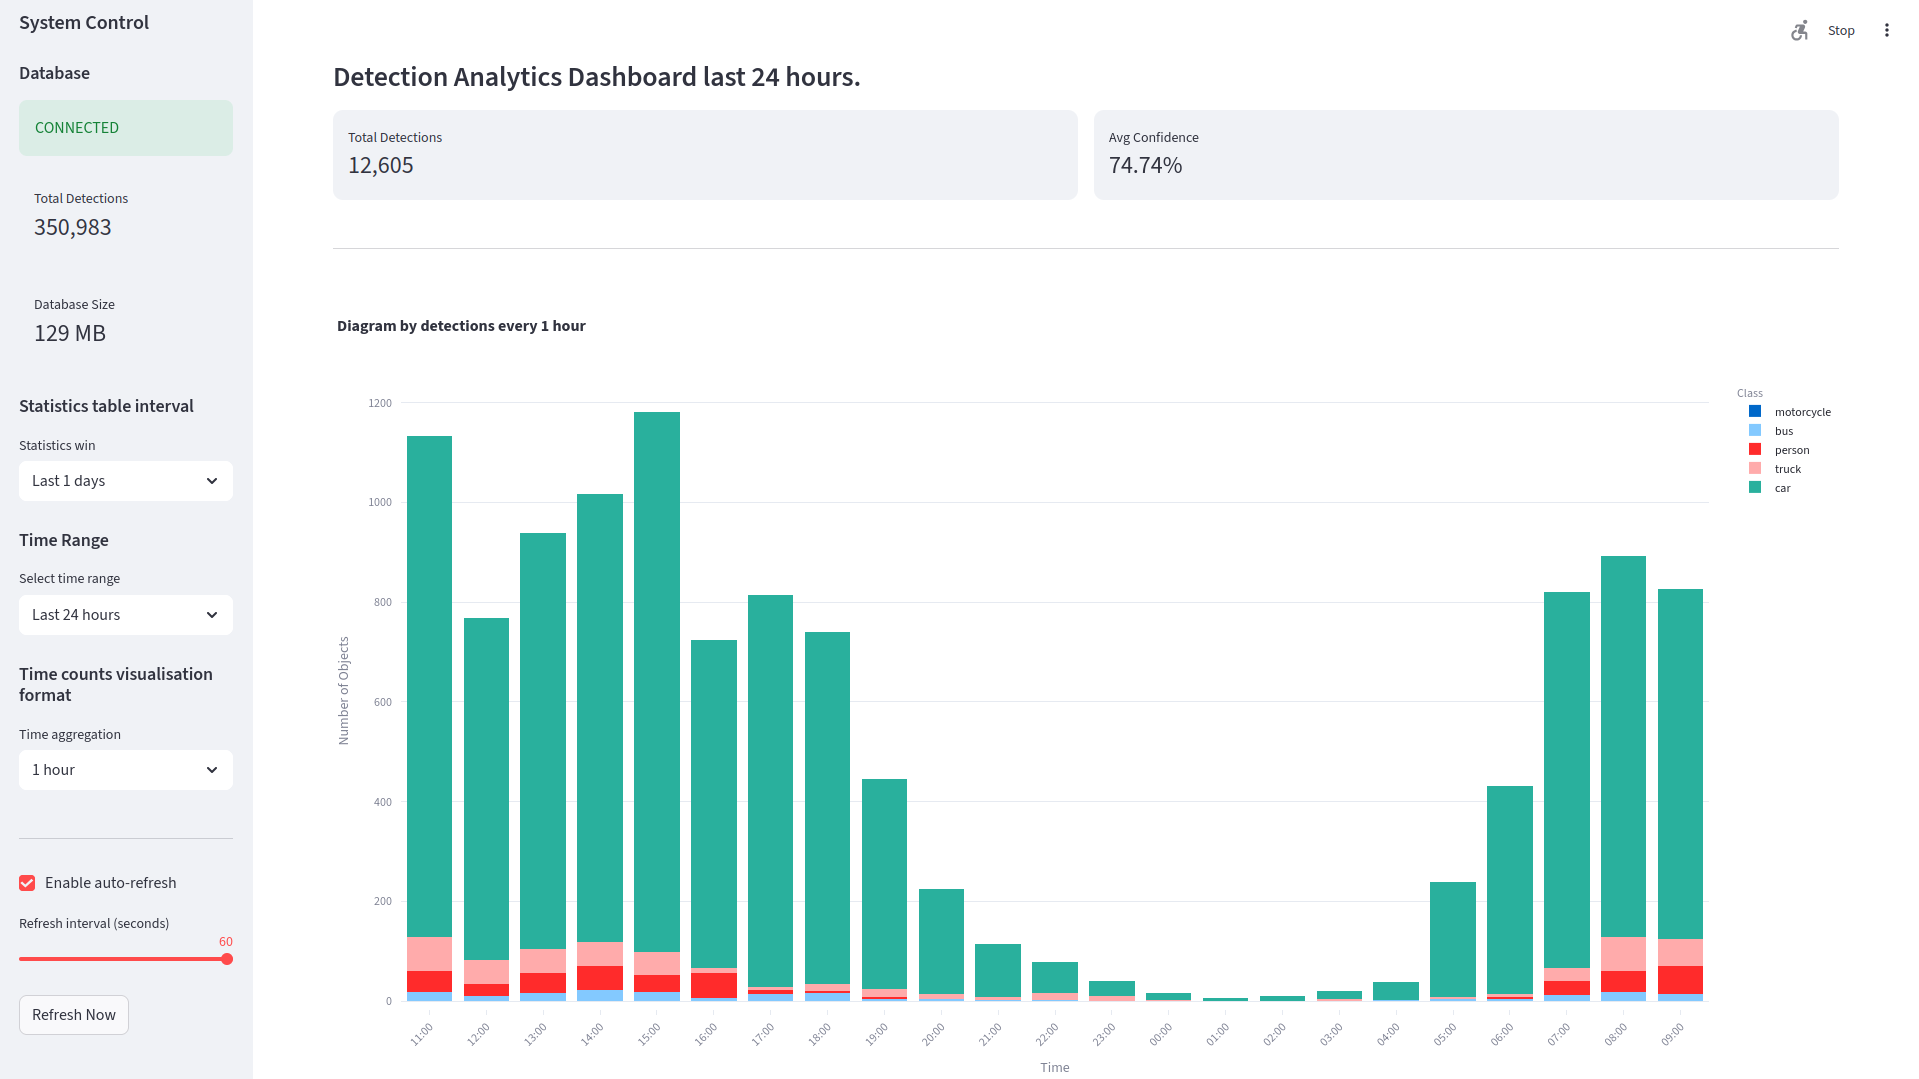
\includegraphics[width=0.95\textwidth]{images/visualisation_dashboard.png}
    \caption{Ukázka implementovaného vizualizačního dashboardu systému.}
    \label{fig:visualisation_dashboard}
\end{figure}

Pro dynamickou analýzu vývoje dopravy v čase využívá aplikace metodu \texttt{resample()}, která umožňuje uživateli měnit šířku časového okna agregace (např. 1~minuta, 10~minut, 1~hodina) jak globálně, tak pro jednotlivé kategorie vozidel (ukázka~\ref{lst:pandas_resample}).

\begin{lstlisting}[language=Python, caption={Časová agregace detekcí podle tříd vozidel v knihovně Pandas.}, label={lst:pandas_resample}]
df_timeline = df.set_index("timestamp")

df_class_timeline = (
    df_timeline.groupby('class_name')
    .resample(selected_interval)
    .size()
    .reset_index(name="count")
)
\end{lstlisting}

Agregovaná časová řada je následně vykreslena pomocí knihovny Plotly jako skládaný sloupcový graf (\textit{stacked bar chart}), který přehledně zobrazuje celkovou intenzitu provozu i poměrné zastoupení jednotlivých typů vozidel v daných časových intervalech (ukázka~\ref{lst:plotly_bar}).

\begin{lstlisting}[language=Python, caption={Generování skládaného sloupcového grafu pomocí knihovny Plotly.}, label={lst:plotly_bar}]
fig = px.bar(
    df_class_timeline,
    x="timestamp",
    y="count",
    color="class_name",
    barmode="stack"
)
\end{lstlisting}

\section{Implementace detekčního modelu}

\subsection{Kompilace modelu pro Hailo akcelerátor}
Pro spuštění modelu YOLOv8 na AI akcelerátoru Hailo
je nutné převést model do formátu HEF (Hailo Executable Format).
Tento proces zahrnuje parsing, optimalizaci (kvantizaci)
a finální kompilaci pomocí nástroje
Hailo Dataflow Compiler (DFC) \cite{hailo_dfc_docs}.


Pro kalibraci modelu lze využít dvě základní možnosti:

\begin{itemize}
    \item veřejně dostupný dataset,
    například dataset COCO (Common Objects in Context)
    \cite{lin_coco_2014},
    \item vlastní kalibrační dataset,
    který obsahuje snímky odpovídající
    cílovému prostředí nasazení modelu.
\end{itemize}

Kalibrační dataset typicky obsahuje
řádově stovky snímků,
které reprezentují distribuci vstupních dat.

V této práci byla využita validační část datasetu
COCO (val2017), která obsahuje přibližně
5\,000 anotovaných snímků \cite{lin_coco_2014}.
Dataset COCO je rozsáhlý veřejný dataset pro úlohy detekce objektů
a obsahuje desítky tříd běžných objektů v reálných scénách
\cite{lin_coco_2014}. 

Kompilace modelu byla provedena pomocí nástroje
\texttt{hailomz}, který je součástí knihovny
Hailo Model Zoo \cite{hailo_model_zoo}.

Proces kompilace zahrnuje několik kroků:

\begin{itemize}
    \item převod ONNX modelu do formátu HAR,
    \item kvantizaci modelu z formátu FP32 na INT8,
    \item optimalizaci alokace výpočetních zdrojů,
    \item generování finálního binárního souboru HEF.
\end{itemize}

Proces optimalizace a kompilace může trvat několik minut
až desítky minut v závislosti na komplexitě modelu,
zvolených optimalizačních parametrech
a výkonu hostitelského systému.
Kompilace je výpočetně náročná a vyžaduje dostatečný výkon
procesoru a adekvátní kapacitu operační paměti.

V případě nedostatečně výkonného lokálního prostředí
je možné proces kompilace realizovat
na vzdáleném vývojovém serveru nebo cloudové infrastruktuře,
která poskytuje dostatečný výpočetní výkon a paměťové prostředky.

Samotná kompilace byla spuštěna příkazem:

\begin{lstlisting}[language=bash, caption={Kompilace modelu YOLOv8 pomocí Hailo Model Zoo}]
hailomz compile yolov8s \
    --hw-arch hailo8 \
    --calib-path ./coco_full \
    --classes 80
\end{lstlisting}

Výsledkem procesu je optimalizovaný HEF soubor,
který je určen pro běh na architektuře Hailo-8.
Kvantizace modelu do formátu INT8 umožňuje výrazné snížení
výpočetní náročnosti při zachování dostatečné detekční přesnosti.

\subsection{Nasazení modelu na zařízení}
Zkompilovaný model ve formátu HEF
je následně využit v detekční pipeline
běžící na zařízení Raspberry Pi~5.
Inference probíhá pomocí běhového prostředí
HailoRT a je akcelerována
AI modulem Hailo.

Tento přístup umožňuje
real-time zpracování video streamu
při zachování nízké spotřeby energie.


\section{Implementace zpracování videa}
\subsection{Kontrukce GStreamer pipeline}
\begin{lstlisting}[language=Python, caption={Zjednodušená konstrukce GStreamer pipeline}]
pipeline_str = (
    "rtspsrc location=rtsp://CAMERA_IP latency=150 "
    "! rtph264depay ! h264parse ! avdec_h264 "
    "! videoconvert ! videoscale "
    "! video/x-raw,width=640,height=640,format=RGB "
    "! hailonet hef-path=<model.hef> batch-size=1 "
    "! hailofilter function-name=yolov8m "
    "! hailotracker iou-thr=0.5 "
    "! videoconvert ! fakesink"
)
\end{lstlisting}

Ukázka demonstruje vytvoření GStreamer pipeline, která provádí:
dekódování RTSP streamu, předzpracování obrazu,
inference modelu YOLO na akcelerátoru Hailo,
post-processing detekcí a sledování objektů.

\subsection{Konfigurace inference a parametry NMS}
Model je spuštěn pomocí prvku \texttt{hailonet}
v rámci GStreamer pipeline.
Inference probíhá nad optimalizovaným HEF souborem,
který je určen pro běh na AI akcelerátoru.

\begin{lstlisting}[language=Python, caption={Konfigurace inference modelu}]
"! hailonet hef-path=model.hef batch-size=1 "
"nms-score-threshold=0.6 nms-iou-threshold=0.5 "
\end{lstlisting}

Parametr \texttt{batch-size=1} zajišťuje,
že každý snímek je zpracován okamžitě bez dávkování.
Parametry \texttt{nms-score-threshold} a \texttt{nms-iou-threshold}
určují chování algoritmu Non-Maximum Suppression (NMS),
který eliminuje překrývající se detekce.


\subsection{Ukázka větvení pipeline (tee)}
\begin{lstlisting}[language=Python, caption={Větvení pipeline pomocí prvku tee}]
pipeline_str += "! tee name=t "
pipeline_str += (
    "t. ! queue ! appsink name=rtsp_sink "
    "t. ! queue ! x264enc ! mp4mux ! filesink location=output.mp4"
)
\end{lstlisting}

Prvek tee umožňuje paralelní zpracování výstupu pipeline, např. současné streamování a ukládání videa.

\subsection{Registrace buffer probe}
\begin{lstlisting}[language=Python, caption={Registrace buffer probe pro získání detekčních dat}]
hailotracker = self.pipeline.get_by_name('hailotracker')
pad = hailotracker.get_static_pad('src')
pad.add_probe(Gst.PadProbeType.BUFFER, self.buffer_probe_callback)
\end{lstlisting}

Buffer probe je využit k zachycení metadat generovaných detekčním a sledovacím modulem.
Tímto mechanismem jsou extrahována detekční data pro další zpracování (počítání průchodů, publikace přes MQTT).

\subsection{Extrakce detekčních metadat}
\begin{lstlisting}[language=Python, caption={Extrakce detekčních metadat z GStreamer bufferu}]
buffer = info.get_buffer()
roi = get_roi_from_buffer(buffer)
hailo_detections = roi.get_objects_typed(HAILO_DETECTION)

for detection in hailo_detections:
    label = detection.get_label()
    confidence = detection.get_confidence()
\end{lstlisting}

Detekční metadata jsou extrahována přímo z GStreamer bufferu pomocí Hailo API, což umožňuje efektivní zpracování bez nutnosti kopírování obrazových dat.

\subsection{Zpracování obrazu v reálném čase}
Zpracování obrazu je navrženo tak, aby systém byl schopen
pracovat v režimu blízkém reálnému času na vestavěném zařízení
s omezeným výpočetním výkonem.

\paragraph{Frame-by-frame zpracování}

Video stream je zpracováván sekvenčně po jednotlivých snímcích
(frame-by-frame). Každý snímek prochází následujícími kroky:
dekódování, předzpracování (změna rozlišení a barevného formátu),
inference detekčního modelu, post-processing a sledování objektů.
Tento přístup umožňuje deterministické chování systému
a průběžnou extrakci detekčních metadat.

\paragraph{Batch size = 1}

Inference modelu je nastavena s parametrem \texttt{batch-size=1}.
Tím je zajištěno, že každý snímek je zpracován okamžitě po přijetí,
bez čekání na naplnění dávky více snímků. 
Toto nastavení minimalizuje latenci mezi vstupem obrazu
a výstupem detekčních výsledků, což je klíčové
pro aplikace dopravního monitoringu.

\paragraph{Použití prvků queue a leaky režimu}

V rámci GStreamer pipeline jsou využity prvky \texttt{queue},
které oddělují jednotlivé fáze zpracování.
U vybraných částí pipeline je aktivován režim
\texttt{leaky=downstream}, který umožňuje zahazování
nejstarších snímků v případě přetížení systému.

Tento mechanismus zabraňuje hromadění snímků ve frontě
a eliminuje postupné narůstání latence,
které by vedlo ke zpožděnému zobrazení detekcí.

\paragraph{Optimalizace latence}

Latence systému je minimalizována kombinací následujících opatření:

\begin{itemize}
    \item zpracování jednotlivých snímků bez dávkování,
    \item omezení velikosti bufferů ve frontách,
    \item využití hardwarové akcelerace inference,
    \item minimalizace kopírování obrazových dat.
\end{itemize}

Tím je dosaženo stabilního a predikovatelného chování
systému i při zvýšeném zatížení.

\paragraph{Využití AI akcelerátoru}

Inference neuronové sítě je realizována pomocí specializovaného
AI akcelerátoru, který umožňuje paralelní výpočet konvolučních
operací přímo na úrovni hardwaru. 
Díky tomu je dosaženo výrazně vyšší rychlosti zpracování
ve srovnání s čistě CPU řešením a je umožněno
nasazení systému na nízkoenergetické edge platformě.

\subsection{Detekce průchodů a průjezdů}
\subsubsection{Polygonální ROI zóna}

\begin{lstlisting}[language=Python, caption={Filtrace detekcí v definované polygonální zóně}]
# Bounding box center determination
cx = bbox.xmin() + bbox.width() * 0.5
cy = bbox.ymin() + bbox.height() * 0.5

# Check if object is in zone
detection_point = Point(cx, cy)
if not self.zone_polygon.contains(detection_point):
    continue
\end{lstlisting}

Detekce jsou filtrovány podle polohy středu bounding boxu.
Pro určení, zda objekt vstoupil do definované oblasti zájmu, je využita polygonální reprezentace detekční zóny pomocí Shapely knihovny.

\subsubsection{Ochrana proti duplicitnímu odesílání track ID}

\begin{lstlisting}[language=Python, caption={Prevence duplicitního odeslání detekcí}]
if tracking_id in self.sent_track_ids:
    continue

self._mark_sent(tracking_id)
\end{lstlisting}

Pro zabránění opakovanému odesílání stejných objektů je využita množina již zpracovaných identifikátorů sledovaných objektů.

\subsubsection{Thread-safe aktualizace detekčních dat}

\begin{lstlisting}[language=Python, caption={Thread-safe aktualizace detekčních dat}]
with self.lock:
    self.detections = detections
    self.frame_count = frame_count
    self.timestamp = datetime.now().isoformat()
\end{lstlisting}

\subsection{Měření výkonnosti (FPS)}

Pro vyhodnocení schopnosti systému zpracovávat video stream
v reálném čase byla implementována metrika
Frames Per Second (FPS), která vyjadřuje počet
zpracovaných snímků za sekundu.

Výpočet FPS je realizován průběžně během běhu pipeline
na základě počtu zpracovaných snímků a uplynulého času:

\[
FPS = \frac{N_{frames}}{t}
\]

kde $N_{frames}$ představuje počet zpracovaných snímků
a $t$ je časový interval v sekundách.

\begin{lstlisting}[language=Python, caption={Průběžný výpočet FPS během běhu pipeline}]
self.frame_count += 1
elapsed_time = time.time() - self.start_time
fps = self.frame_count / elapsed_time
\end{lstlisting}

Hodnota FPS je využívána jako indikátor výkonnosti
celé detekční pipeline a umožňuje ověřit,
zda systém splňuje požadavky na real-time zpracování.
Díky využití hardwarového akcelerátoru
je dosaženo stabilního průběhu zpracování
bez významných výkyvů výkonu.



\section{Ukládání a vizualizace dat}
\subsection{Přenos detekčních dat pomocí MQTT}
Pro přenos detekčních událostí mezi edge zařízením a backendovou
částí systému je využit protokol MQTT. 
Tento protokol je vhodný pro lehkou a asynchronní komunikaci
v distribuovaných systémech, zejména v prostředí IoT.

V navržené architektuře je detekční pipeline
zcela oddělena od databázové vrstvy.
Edge zařízení publikuje detekční data do MQTT brokeru,
zatímco samostatný subscriber modul
zajišťuje jejich následné uložení do databáze.

Každá detekce je reprezentována strukturou obsahující
následující atributy:

\begin{itemize}
    \item \textbf{class\_id} – numerický identifikátor třídy,
    \item \textbf{class\_name} – název detekovaného objektu,
    \item \textbf{confidence} – pravděpodobnost detekce,
    \item \textbf{bbox} – souřadnice ohraničujícího obdélníku,
    \item \textbf{track\_id} – identifikátor sledovaného objektu,
    \item \textbf{timestamp} – čas detekce.
\end{itemize}

\begin{lstlisting}[language=Python, caption={Odesílání dat z pipeline do MQTT}]
detection_dict = {
    "class_id": class_id,
    "class_name": label,
    "confidence": float(confidence),
    "bbox": bbox_coords,
    "track_id": tracking_id,
    "timestamp": current_timestamp
}

detection_list.append(detection_dict)

if detection_list and self.mqtt_publisher.connected:
    self.mqtt_publisher.publish(detection_list)
\end{lstlisting}

Ze získaných detekčních metadat se vytvoří slovník kam se uloží aktuální detekce. 

Publikace zprávy probíhá pouze v případě,
že je seznam detekcí neprázdný
a spojení s MQTT brokerem je aktivní.
Tím je zajištěno, že do komunikační vrstvy
nejsou odesílány redundantní nebo neúplné informace.

Databázový modul je implementován jako samostatný MQTT subscriber,
který přijímá publikované zprávy
a ukládá je do relační databáze PostgreSQL.

Tento přístup umožňuje oddělení real-time inference
od operací zápisu do databáze,
čímž je minimalizováno riziko zpomalení detekční části systému.

Identifikátor \textit{track\_id} je označen jako zpracovaný
až po úspěšném odeslání zprávy.

Tím je zabráněno situaci,
kdy by byla detekce považována za odeslanou,
aniž by skutečně došlo k jejímu předání
komunikační vrstvě.

\subsection{Ukládání detekčních událostí}
Detekční události jsou po přijetí prostřednictvím MQTT
zpracovány a následně ukládány do relační databáze PostgreSQL.
Pro zajištění efektivního a škálovatelného přístupu
je využit mechanismus connection poolingu,
který umožňuje opakované využívání databázových spojení
bez nutnosti jejich opětovného vytváření.

Pro zvýšení výkonu při vysokém počtu detekcí
je implementováno dávkové ukládání (batch insert),
které umožňuje vložení více záznamů v rámci jedné transakce.

\begin{lstlisting}[language=Python, caption={Dávkové ukládání detekcí do databáze}]
query = """
INSERT INTO detections
(timestamp_, frame_id, class_name, confidence, x1, y1, x2, y2, track_id)
VALUES (%s, %s, %s, %s, %s, %s, %s, %s, %s)
"""
execute_batch(cursor, query, data, page_size=100)
conn.commit()
\end{lstlisting}


\subsection{Vizualizační rozhraní}
Vizualizační rozhraní systému je realizováno jako interaktivní
dashboard umožňující časovou analýzu detekcí,
agregaci podle tříd objektů a prostorovou analýzu.

\begin{figure}[H]
    \centering
    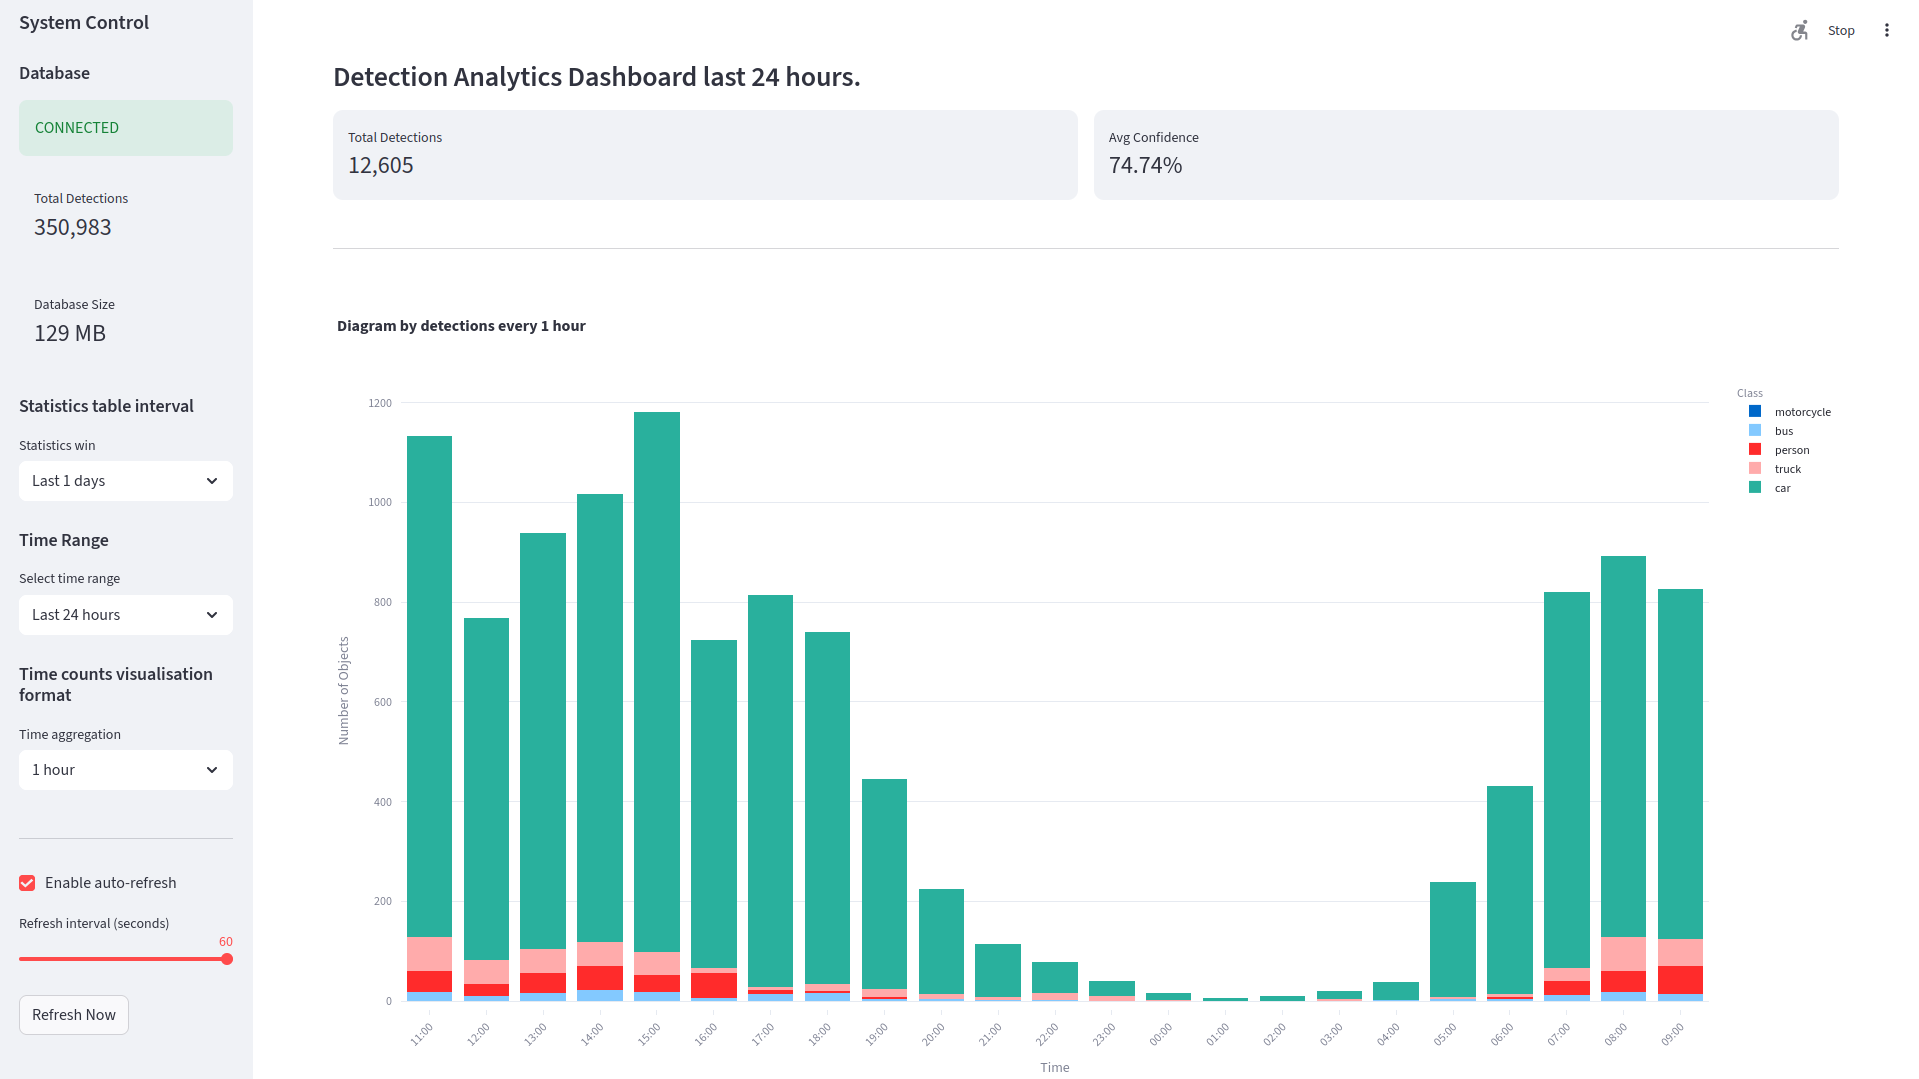
\includegraphics[width=0.95\textwidth]{images/visualisation_dashboard.png}
    \caption{Ukázka vizualizačního dashboardu systému}
    \label{fig:visualisation_dashboard}
\end{figure}

Dashboard poskytuje přehled o celkovém počtu detekcí,
průměrné hodnotě confidence a umožňuje volbu časového intervalu
pro agregaci dat.

\subsubsection{Načítání a transformace dat}
Data jsou načítána z databáze pomocí API endpointů
(\texttt{/api/detections}, \texttt{/api/statistics})
a následně transformována do datového rámce knihovny Pandas.
Součástí transformace je převod časových údajů na formát \texttt{datetime}
a rozbalení souřadnic ohraničujících obdélníků (bounding box) do samostatných
sloupců.

\subsubsection{Časová agregace detekcí}
Pro analýzu časového vývoje detekcí je využita metoda
\texttt{resample()}, která umožňuje agregaci dat
do různých časových intervalů (např. 1 minuta, 10 minut, 1 hodina).
Agregace je realizována jak globálně, tak i samostatně
pro jednotlivé třídy objektů.

\begin{lstlisting}[language=Python, caption={Časová agregace detekcí podle tříd}]
df_timeline = df.set_index("timestamp")

df_class_timeline = (
    df_timeline.groupby('class_name')
    .resample(selected_interval)
    .size()
    .reset_index(name="count")
)
\end{lstlisting}

Tento přístup umožňuje dynamickou změnu velikosti časového intervalu
a poskytuje flexibilní nástroj pro analýzu dopravní zátěže
v různých časových měřítkách.

\subsubsection{Stacked časová vizualizace}

Pro zobrazení časového vývoje detekcí podle tříd objektů
je využit stacked bar graf, který umožňuje
současné zobrazení více kategorií v rámci jednoho časového intervalu.

\begin{lstlisting}[language=Python, caption={Stacked bar graf časové agregace}]
fig = px.bar(
    df_class_timeline,
    x="timestamp",
    y="count",
    color="class_name",
    barmode="stack"
)
\end{lstlisting}

Tento typ vizualizace umožňuje identifikovat časové špičky,
porovnat relativní zastoupení jednotlivých tříd
a analyzovat změny dopravního zatížení v průběhu dne.

\chapter{Testování a vyhodnocení}
Pro vyhodnocení navrženého systému byla použita
stejná video sekvence zachycující dopravní situaci
za špatných zimních a povětrnostních podmínek (sněžení).
Byla analyzována čtyřminutová část videa,
která byla zvolena jako reprezentativní
z delšího záznamu. 

Vyhodnocení bylo provedeno na dvou odlišných platformách.:

\begin{itemize}
    \item \textbf{Edge řešení (Hailo)} – detekce probíhala na zařízení
    Raspberry Pi 5 s využitím AI akcelerátoru Hailo,
    modelu YOLOv8m a sledovacího modulu \textit{hailotracker}.
    \item \textbf{GPU řešení} – detekce byla realizována
    na osobním počítači s GPU s využitím knihoven
    Ultralytics a OpenCV, modelu YOLOv11l
    a sledovacího algoritmu ByteTrack.
\end{itemize}

Detekční systém běžící na zařízení Raspberry Pi 5
je zároveň navržen jako kontinuální real-time aplikace, která nepřetržitě zpracovává video stream 
a vrací detekční události.

Získaná data jsou průběžně odesílána
prostřednictvím MQTT protokolu do backendové části systému,
kde jsou ukládána do databáze
a následně vizualizována v podobě interaktivního dashboardu.
Tento přístup umožňuje dlouhodobý sběr dat
a analýzu dopravních statistik v reálném čase.

Experimentální vyhodnocení bylo provedeno offline,
zatímco edge řešení je v praxi provozováno
v nepřetržitém režimu.

\section{Testovací scénáře}

Pro vyhodnocení navrženého systému byla použita
stejná video sekvence zachycující dopravní situaci
v zimních podmínkách (sněžení).

Video bylo analyzováno dvěma přístupy:
\begin{itemize}
    \item \textbf{Edge řešení (Hailo)} – detekce pomocí modelu YOLOv8m
    optimalizovaného pro akcelerátor Hailo a běžícího na zařízení Raspberry Pi 5.
    Pro sledování objektů byl využit modul \textit{hailotracker}
    v rámci GStreamer pipeline.

    \item \textbf{GPU řešení} – detekce pomocí modelu YOLOv11l
    realizovaná na osobním počítači s GPU,
    s využitím knihoven Ultralytics a OpenCV.
    Pro sledování objektů byl použit algoritmus ByteTrack.
\end{itemize}

Pro vyhodnocení přesnosti byla vytvořena referenční
hodnota (ground truth), která byla získána manuálním
počítáním objektů ve vybrané části video sekvence.

Pro oba přístupy byly definovány oblasti zájmu (ROI),
které se mírně lišily:

\begin{itemize}
    \item u Hailo řešení byla použita polygonální ROI,
    která byla zmenšena z důvodu omezení výskytu duplicitních detekcí,
    \item u GPU řešení byla použita obdélníková ROI,
    kde se problém ghostingu nevyskytoval v takové míře.
\end{itemize}

\section{Vyhodnocení přesnosti detekce}
Přesnost detekce byla vyhodnocena pomocí metriky accuracy.

Pro vyhodnocení detekční schopnosti byly analyzovány
výstupy obou modelů ve formě počtu detekovaných objektů
a jejich shody s referenčními hodnotami.

Výsledky pro Hailo řešení ukazují,
že bylo detekováno celkem 127 unikátních objektů
při průměrné confidence přibližně 0.77 pro třídu \textit{car}

GPU řešení detekovalo celkem 132 unikátních objektů
s průměrnou confidence přibližně 0.76 pro třídu \textit{car}


Oba modely vykazují srovnatelnou detekční přesnost,
přičemž GPU řešení dosahuje mírně vyššího počtu detekcí,
což může být způsobeno vyšší citlivostí modelu
a menším vlivem optimalizace pro edge zařízení. Jejich celková průměrná accuracy je 0.73 u GPU a 0.74 u Hailo.

\section{Vyhodnocení přesnosti sčítání}
Na základě porovnání s ručně anotovanými daty dosáhlo GPU řešení vyšší přesnosti,
zatímco Hailo řešení vykazovalo vyšší míru chyb způsobenou zejména duplicitními detekcemi (ghosting). Přesnost byla hodnocena na základě absolutní odchylky
a relativní chyby vůči ground truth.

\begin{table}[H]
\centering
\begin{tabular}{|l|c|c|c|}
\hline
\textbf{Třída} & \textbf{Hailo AI} & \textbf{GPU} & \textbf{Ruční (GT)} \\
\hline
Car & 120 & 108 & 108 \\
Bus & 4 & 11 & 3 \\
Truck & 3 & 12 & 6 \\
Person & 1 & 0 & 1 \\

\hline
\textbf{Celkem} & 127 & 132 & 118 \\
\hline
\end{tabular}
\caption{Porovnání počtu detekovaných objektů}
\end{table}

Z tabulky vyplývá,
že GPU řešení dosahuje vyšší přesnosti,
zejména u třídy \textit{Car},
kde přesně odpovídá ručnímu měření.

Naopak řešení založené na akcelerátoru Hailo
vykazuje vyšší odchylku od ground truth,
především v důsledku duplicitních detekcí
(ghosting efekt),
kdy je jeden objekt započítán vícekrát.

U tříd \textit{Bus} a \textit{Truck}
jsou patrné výraznější rozdíly mezi jednotlivými metodami,
což může být způsobeno menším počtem vzorků
a vyšší citlivostí na chybné detekce.

Celkově lze konstatovat,
že GPU řešení poskytuje přesnější výsledky,
zatímco Hailo řešení vykazuje vyšší chybu sčítání,
která je však vyvážena nižší latencí
a vyšší energetickou efektivitou.

Pro kvantitativní vyhodnocení přesnosti sčítání byla použita
metrika přesnosti sčítání (\textit{counting accuracy}),
která porovnává počet objektů určený systémem
s ručně stanovenou referenční hodnotou (ground truth):

\[
Accuracy_{count} =
\left(
1 - \frac{|N_{real}-N_{sys}|}{N_{real}}
\right)\cdot 100 \%
\]

kde $N_{real}$ představuje skutečný počet objektů
získaný ruční anotací a $N_{sys}$ počet objektů
detekovaných systémem.

Na základě metriky přesnosti sčítání dosáhlo řešení
s akcelerátorem Hailo hodnoty 92{,}37 \%,
zatímco GPU řešení dosáhlo 88{,}14 \%.

Přestože GPU řešení vykazovalo přesnější klasifikaci
některých jednotlivých tříd objektů,
celkový počet detekovaných objektů byl bližší
referenční hodnotě u řešení založeného na akcelerátoru Hailo.
Rozdíly mezi metodami byly způsobeny zejména
chybami sledování objektů a vznikem duplicitních detekcí.

\section{Vyhodnocení výkonnosti systému}
Výkonnost systému byla hodnocena z hlediska schopnosti real-time zpracování video streamu.

Edge řešení s využitím akcelerátoru Hailo umožňuje
spuštění detekce přímo na zařízení Raspberry Pi,
čímž odpadá nutnost přenosu dat do cloudu.

GPU řešení poskytuje vyšší flexibilitu
a přesnost detekce, avšak za cenu vyšších
hardwarových nároků.

Hlavní výhodou edge přístupu je nízká latence
a nezávislost na síťové konektivitě.

- dosažené FPS
- latence
- využití CPU
- vliv akcelerátoru

\chapter{Diskuze a prezentace výsledků}
Výsledky ukazují, že oba přístupy mají své výhody
i omezení.

Hailo řešení umožňuje efektivní real-time zpracování
na edge zařízení s nízkou spotřebou energie,
avšak může docházet k chybám způsobeným optimalizací modelu
a omezenou přesností kvantizace.

GPU řešení dosahuje vyšší přesnosti detekce
a stabilnějšího sledování objektů,
zejména díky použití pokročilejšího modelu
a robustnějšího tracking algoritmu.

Rozdíly v přesnosti byly také ovlivněny
rozdílnou definicí ROI oblastí,
kde menší polygonální oblast u Hailo řešení
byla zvolena za účelem redukce chyb způsobených ghostingem.

\chapter{Závěr}
- Shrnutí dosažených cílů.
- Zhodnocení přínosu a praktické využitelnosti práce.
- Návrhy na další rozšíření a vylepšení.

\sloppy
\printbibliography[title=Seznam použitých zdrojů]
\cite{harris_numpy_2020}
\cite{hyndman_forecasting_2018}
\cite{li_edge_ai_2020}
\cite{mckinney_pandas_2010}
\cite{mqtt_oasis_2019}
\cite{plotly_docs_2015}
\cite{psycopg_docs_2025}
\cite{python_docs_313_2025}
\cite{raspberrypi_ai_kit}
\cite{raspberrypi_docs_2024}
\cite{redmon_yolo_2016}
\cite{szeliski_computer_vision}
\cite{zhou_traffic_survey_2024}

\appendix

\chapter{Externí přílohy\label{sec:ep}}

V této kapitole stačí uvést pouze základní strukturu úložiště (co se kde nalézá a jakou má funkci) například v podobě tabulky. 

\begin{longtable}{ll}
\hline
ki-thesis.pdf & text práce v PDF \\
ki-thesis.tex & zdrojový kód práce v \LaTeX{}u \\
kitheses.cls & definice třídy dokumentů (rozšířená třída \texttt{scrbook} \\
thesis.bib & bibliografická databáze (exportována z citace.com) \\
LOGO\_PRF\_CZ\_RGB\_standard.jpg  & logo fakulty s českým textem \\
LOGO\_PRF\_EM\_RGB\_standard.jpg  & logo fakulty s anglickým textem  \\
\hline
\end{longtable}

Všechny tyto soubory jsou potřeba pro překlad dokumentu (logo stačí jedno v příslušné jazykové verzi).


\end{document}

